\documentclass[onecolumn,prx,amsmath,amssymb,12pt]{revtex4-2}
\usepackage{enumitem}
\usepackage{graphicx}
\usepackage{float}
\usepackage{amssymb,amsthm,amsfonts,amstext}
\usepackage{url}
\usepackage{color}
\usepackage{xcolor}
\usepackage{bbm}
%\usepackage[lite]{mtpro2}
\usepackage{changes}
\usepackage{lipsum}
\usepackage{mathrsfs}
\usepackage{qcircuit}

\usepackage{calrsfs}
\DeclareMathAlphabet{\pazocal}{OMS}{zplm}{m}{n}
%\usepackage{amsmath,amsthm,amscd,amssymb}
\usepackage[colorlinks=true
,breaklinks=true
,urlcolor=blue
,anchorcolor=blue
,citecolor=blue
,filecolor=blue
,linkcolor=blue
,menucolor=blue
,linktocpage=true]{hyperref}
\hypersetup{
bookmarksopen=true,
bookmarksnumbered=true,
bookmarksopenlevel=10
}
\usepackage[noBBpl,sc]{mathpazo}
\usepackage[papersize={7.0in, 10.0in}, left=.5in, right=.5in, top=1in, bottom=.9in]{geometry}
\linespread{1.1}
\sloppy
\raggedbottom
\pagestyle{plain}
\usepackage{microtype}

% these include amsmath and that can cause trouble in older docs.
\makeatletter
\@ifpackageloaded{amsmath}{}{\RequirePackage{amsmath}}

\DeclareFontFamily{U}  {cmex}{}
\DeclareSymbolFont{Csymbols}       {U}  {cmex}{m}{n}
\DeclareFontShape{U}{cmex}{m}{n}{
    <-6>  cmex5
   <6-7>  cmex6
   <7-8>  cmex6
   <8-9>  cmex7
   <9-10> cmex8
  <10-12> cmex9
  <12->   cmex10}{}

\def\Set@Mn@Sym#1{\@tempcnta #1\relax}
\def\Next@Mn@Sym{\advance\@tempcnta 1\relax}
\def\Prev@Mn@Sym{\advance\@tempcnta-1\relax}
\def\@Decl@Mn@Sym#1#2#3#4{\DeclareMathSymbol{#2}{#3}{#4}{#1}}
\def\Decl@Mn@Sym#1#2#3{%
  \if\relax\noexpand#1%
    \let#1\undefined
  \fi
  \expandafter\@Decl@Mn@Sym\expandafter{\the\@tempcnta}{#1}{#3}{#2}%
  \Next@Mn@Sym}
\def\Decl@Mn@Alias#1#2#3{\Prev@Mn@Sym\Decl@Mn@Sym{#1}{#2}{#3}}
\let\Decl@Mn@Char\Decl@Mn@Sym
\def\Decl@Mn@Op#1#2#3{\def#1{\DOTSB#3\slimits@}}
\def\Decl@Mn@Int#1#2#3{\def#1{\DOTSI#3\ilimits@}}

\let\sum\undefined
\DeclareMathSymbol{\tsum}{\mathop}{Csymbols}{"50}
\DeclareMathSymbol{\dsum}{\mathop}{Csymbols}{"51}

\Decl@Mn@Op\sum\dsum\tsum

\makeatother

\makeatletter
\@ifpackageloaded{amsmath}{}{\RequirePackage{amsmath}}

\DeclareFontFamily{OMX}{MnSymbolE}{}
\DeclareSymbolFont{largesymbolsX}{OMX}{MnSymbolE}{m}{n}
\DeclareFontShape{OMX}{MnSymbolE}{m}{n}{
    <-6>  MnSymbolE5
   <6-7>  MnSymbolE6
   <7-8>  MnSymbolE7
   <8-9>  MnSymbolE8
   <9-10> MnSymbolE9
  <10-12> MnSymbolE10
  <12->   MnSymbolE12}{}

\DeclareMathSymbol{\downbrace}    {\mathord}{largesymbolsX}{'251}
\DeclareMathSymbol{\downbraceg}   {\mathord}{largesymbolsX}{'252}
\DeclareMathSymbol{\downbracegg}  {\mathord}{largesymbolsX}{'253}
\DeclareMathSymbol{\downbraceggg} {\mathord}{largesymbolsX}{'254}
\DeclareMathSymbol{\downbracegggg}{\mathord}{largesymbolsX}{'255}
\DeclareMathSymbol{\upbrace}      {\mathord}{largesymbolsX}{'256}
\DeclareMathSymbol{\upbraceg}     {\mathord}{largesymbolsX}{'257}
\DeclareMathSymbol{\upbracegg}    {\mathord}{largesymbolsX}{'260}
\DeclareMathSymbol{\upbraceggg}   {\mathord}{largesymbolsX}{'261}
\DeclareMathSymbol{\upbracegggg}  {\mathord}{largesymbolsX}{'262}
\DeclareMathSymbol{\braceld}      {\mathord}{largesymbolsX}{'263}
\DeclareMathSymbol{\bracelu}      {\mathord}{largesymbolsX}{'264}
\DeclareMathSymbol{\bracerd}      {\mathord}{largesymbolsX}{'265}
\DeclareMathSymbol{\braceru}      {\mathord}{largesymbolsX}{'266}
\DeclareMathSymbol{\bracemd}      {\mathord}{largesymbolsX}{'267}
\DeclareMathSymbol{\bracemu}      {\mathord}{largesymbolsX}{'270}
\DeclareMathSymbol{\bracemid}     {\mathord}{largesymbolsX}{'271}

\def\horiz@expandable#1#2#3#4#5#6#7#8{%
  \@mathmeasure\z@#7{#8}%
  \@tempdima=\wd\z@
  \@mathmeasure\z@#7{#1}%
  \ifdim\noexpand\wd\z@>\@tempdima
    $\m@th#7#1$%
  \else
    \@mathmeasure\z@#7{#2}%
    \ifdim\noexpand\wd\z@>\@tempdima
      $\m@th#7#2$%
    \else
      \@mathmeasure\z@#7{#3}%
      \ifdim\noexpand\wd\z@>\@tempdima
        $\m@th#7#3$%
      \else
        \@mathmeasure\z@#7{#4}%
        \ifdim\noexpand\wd\z@>\@tempdima
          $\m@th#7#4$%
        \else
          \@mathmeasure\z@#7{#5}%
          \ifdim\noexpand\wd\z@>\@tempdima
            $\m@th#7#5$%
          \else
           #6#7%
          \fi
        \fi
      \fi
    \fi
  \fi}

\def\overbrace@expandable#1#2#3{\vbox{\m@th\ialign{##\crcr
  #1#2{#3}\crcr\noalign{\kern2\p@\nointerlineskip}%
  $\m@th\hfil#2#3\hfil$\crcr}}}
\def\underbrace@expandable#1#2#3{\vtop{\m@th\ialign{##\crcr
  $\m@th\hfil#2#3\hfil$\crcr
  \noalign{\kern2\p@\nointerlineskip}%
  #1#2{#3}\crcr}}}

\def\overbrace@#1#2#3{\vbox{\m@th\ialign{##\crcr
  #1#2\crcr\noalign{\kern2\p@\nointerlineskip}%
  $\m@th\hfil#2#3\hfil$\crcr}}}
\def\underbrace@#1#2#3{\vtop{\m@th\ialign{##\crcr
  $\m@th\hfil#2#3\hfil$\crcr
  \noalign{\kern2\p@\nointerlineskip}%
  #1#2\crcr}}}

\def\bracefill@#1#2#3#4#5{$\m@th#5#1\leaders\hbox{$#4$}\hfill#2\leaders\hbox{$#4$}\hfill#3$}

\def\downbracefill@{\bracefill@\braceld\bracemd\bracerd\bracemid}
\def\upbracefill@{\bracefill@\bracelu\bracemu\braceru\bracemid}

\DeclareRobustCommand{\downbracefill}{\downbracefill@\textstyle}
\DeclareRobustCommand{\upbracefill}{\upbracefill@\textstyle}

\def\upbrace@expandable{%
  \horiz@expandable
    \upbrace
    \upbraceg
    \upbracegg
    \upbraceggg
    \upbracegggg
    \upbracefill@}
\def\downbrace@expandable{%
  \horiz@expandable
    \downbrace
    \downbraceg
    \downbracegg
    \downbraceggg
    \downbracegggg
    \downbracefill@}

\DeclareRobustCommand{\overbrace}[1]{\mathop{\mathpalette{\overbrace@expandable\downbrace@expandable}{#1}}\limits}
\DeclareRobustCommand{\underbrace}[1]{\mathop{\mathpalette{\underbrace@expandable\upbrace@expandable}{#1}}\limits}

\makeatother


\usepackage[small]{titlesec}

% make sure there is enough TOC for reasonable pdf bookmarks.
\setcounter{tocdepth}{3}

%\usepackage[dotinlabels]{titletoc}
%\titlelabel{{\thetitle}.\quad}
%\usepackage{titletoc}
\usepackage[small]{titlesec}

\titleformat{\section}[block]
  {\fillast\medskip}
  {\bfseries{\thesection. }}
  {1ex minus .1ex}
  {\bfseries}
 
\titleformat*{\subsection}{\itshape}
\titleformat*{\subsubsection}{\itshape}

\setcounter{tocdepth}{2}

\titlecontents{section}
              [2.3em] 
              {\bigskip}
              {{\contentslabel{2.3em}}}
              {\hspace*{-2.3em}}
              {\titlerule*[1pc]{}\contentspage}
              
\titlecontents{subsection}
              [4.7em] 
              {}
              {{\contentslabel{2.3em}}}
              {\hspace*{-2.3em}}
              {\titlerule*[.5pc]{}\contentspage}

% hopefully not used.           
\titlecontents{subsubsection}
              [7.9em]
              {}
              {{\contentslabel{3.3em}}}
              {\hspace*{-3.3em}}
              {\titlerule*[.5pc]{}\contentspage}
%\makeatletter
\renewcommand\tableofcontents{%
    \section*{\contentsname
        \@mkboth{%
           \MakeLowercase\contentsname}{\MakeLowercase\contentsname}}%
    \@starttoc{toc}%
    }
\def\@oddhead{{\scshape\rightmark}\hfil{\small\scshape\thepage}}%
\def\sectionmark#1{%
      \markright{\MakeLowercase{%
        \ifnum \c@secnumdepth >\m@ne
          \thesection\quad
        \fi
        #1}}}
        
\makeatother

\makeatletter

 \def\small{%
  \@setfontsize\small\@xipt{13pt}%
  \abovedisplayskip 8\p@ \@plus3\p@ \@minus6\p@
  \belowdisplayskip \abovedisplayskip
  \abovedisplayshortskip \z@ \@plus3\p@
  \belowdisplayshortskip 6.5\p@ \@plus3.5\p@ \@minus3\p@
  \def\@listi{%
    \leftmargin\leftmargini
    \topsep 9\p@ \@plus3\p@ \@minus5\p@
    \parsep 4.5\p@ \@plus2\p@ \@minus\p@
    \itemsep \parsep
  }%
}%
 \def\footnotesize{%
  \@setfontsize\footnotesize\@xpt{12pt}%
  \abovedisplayskip 10\p@ \@plus2\p@ \@minus5\p@
  \belowdisplayskip \abovedisplayskip
  \abovedisplayshortskip \z@ \@plus3\p@
  \belowdisplayshortskip 6\p@ \@plus3\p@ \@minus3\p@
  \def\@listi{%
    \leftmargin\leftmargini
    \topsep 6\p@ \@plus2\p@ \@minus2\p@
    \parsep 3\p@ \@plus2\p@ \@minus\p@
    \itemsep \parsep
  }%
}%
\def\open@column@one#1{%
 \ltxgrid@info@sw{\class@info{\string\open@column@one\string#1}}{}%
 \unvbox\pagesofar
 \@ifvoid{\footsofar}{}{%
  \insert\footins\bgroup\unvbox\footsofar\egroup
  \penalty\z@
 }%
 \gdef\thepagegrid{one}%
 \global\pagegrid@col#1%
 \global\pagegrid@cur\@ne
 \global\count\footins\@m
 \set@column@hsize\pagegrid@col
 \set@colht
}%

\def\frontmatter@abstractheading{%
\bigskip
 \begingroup
  \centering\large
  \abstractname
  \par\bigskip
 \endgroup
}%

\makeatother

%\DeclareSymbolFont{CMlargesymbols}{OMX}{cmex}{m}{n}
%\DeclareMathSymbol{\sum}{\mathop}{CMlargesymbols}{"50}

\newcommand\setItemnumber[1]{\setcounter{enumi}{\numexpr#1-1\relax}}



\newtheorem{thm}{Theorem}
\newtheorem{cor}{Corollary}
\newtheorem{lem}{Lemma}

\newcommand{\Z}{\mathbb{Z}}
\newcommand{\R}{\mathbb{R}}
\newcommand{\Qset}{\mathcal{Q}}
\newcommand{\Qreal}{\mathcal{Q}_r}
\newcommand{\idm}{\mathbb{1}}
\newcommand{\st}{\hspace{1mm} | \hspace{1mm}}
\def\be{\begin{equation}}
\def\ee{\end{equation}}
\def\bra#1{\langle#1|} \def\ket#1{|#1\rangle}
\def\braket#1#2{\langle#1|#2\rangle}
\def\bracket#1#2{\langle#1,#2\rangle}
\def\ketbra#1#2{\ket{#1}\!\bra{#2}}
\def\proj#1{\ket{#1}\!\bra{#1}}
\def\ve#1{\langle#1\rangle}
\def\id{{\mathbb I}}
\def\tr{\mbox{tr}}
\def\A{{\pazocal A}}
\def\C{{\pazocal C}}
\def\H{{\cal H}}
\newcommand{\miguel}[1]{{\color{red}[MIGUEL: #1]}}
\newcommand{\thinh}[1]{{\color{blue}[THINH: #1]}}
\newcommand{\marco}[1]{{\color{magenta}[MARCO: #1]}}
\newcommand{\armin}[1]{{\color{teal}[ARMIN: #1]}}
\def\norm#1{\| #1 \| }
\def\abs#1{|#1|}

\newcommand{\mirjam}[1]{{\color{purple}[MIRJAM: #1]}}
\newcommand{\david}[1]{{\color{orange}[DAVID: #1]}}
\newcommand{\toni}[1]{{\color{olive}[TONI: #1]}}


\newtheorem{theo}{Theorem}
\newtheorem{remark}{Remark}
\newtheorem{defin}[theo]{Definition}
\newtheorem{obs}[theo]{Observation}
\newtheorem{crit}[theo]{Criterion}
\newtheorem{lemma}[theo]{Lemma}
\newtheorem{prop}[theo]{Proposition}


%\date{November 2020}

\begin{document}


\title{\large Quantum physics needs complex numbers}
\author{\normalsize Marc-Olivier Renou$^1$, David Trillo$^2$, Mirjam Weilenmann$^2$, Le Phuc Thinh$^2$, Armin Tavakoli$^2$, Nicolas Gisin$^{3,4}$, Antonio Ac\'in$^{1,5}$ and Miguel Navascu\'es$^2$}

\affiliation{$^1$ICFO-Institut de Ciencies Fotoniques, The Barcelona Institute of Science and Technology, 08860 Castelldefels (Barcelona), Spain\\
$^2$Institute for Quantum Optics and Quantum Information (IQOQI) Vienna, Austrian Academy of Sciences\\
$^3$Group of Applied Physics, University of Geneva, 1211 Geneva, Switzerland\\
$^4$SIT, Geneva, Switzerland\\
$^5$ICREA-Instituci\`o Catalana de Recerca i Estudis Avançats, Lluis Companys 23, 08010 Barcelona, Spain}


\begin{abstract}
Complex numbers, i.e., numbers with a real and an imaginary part, are essential for mathematical analysis, while their role in other subjects, such as electromagnetism or special relativity, is far less fundamental. Quantum physics is the only physical theory where these numbers seem to play an indispensible role, as the theory is explicitly formulated in terms of operators acting on complex Hilbert spaces. The occurrence of complex numbers within the quantum formalism has nonetheless puzzled countless physicists, including the fathers of the theory, for whom a real version of quantum physics, where states and observables are represented by real operators, seemed much more natural. In fact, previous works showed that such ``real quantum physics'' can reproduce the outcomes of any multipartite experiment, as long as the parts share arbitrary real quantum states. Thus, are complex numbers really needed for a quantum description of nature? Here, we show this to be case by proving that real and complex quantum physics make different predictions in network scenarios comprising independent quantum state sources. This allows us to devise a Bell-type quantum experiment whose input-output correlations cannot be approximated by any real quantum model. The successful realization of such an experiment would disprove real quantum physics, in the same way as standard Bell experiments disproved local  physics.
\end{abstract}
\date{26 Jan 2021}

\maketitle
\newpage

\begin{quote}
\emph{What is unpleasant here, and indeed directly to be objected to, is the use of complex numbers. $\Psi$ is surely fundamentally a real function.}

Letter from Schr\"{o}dinger to Lorentz \cite{einstein2011letters}. June $6^{th}$, 1926.    
\end{quote}

\newpage

Numbers are there to count. Initially, to count sheep and hectares: $1,2,3,...$. Such considerations gave birth to the notion of natural as well as rational numbers. From the middle ages into the renaissance, these numbers were extended into what is known today as the real numbers; that is numbers with any sequence of digits after the dot. With the arrival of Newton and Leibniz, real numbers enabled the invention of calculus to compute changes in the position and velocity of objects. Meanwhile, mathematicians had started playing with numbers for the sake of their beauty. Solutions of simple equations like, e.g. $x^2=2$, had introduced irrational numbers in the Classical Greece. How about $x^2=-1$? At first sight, this equation has no solution, because the square of a real number cannot be negative. Equations without solutions are, however, inconvenient. Hence, mathematicians invented new numbers, today known as complex numbers.

The history of complex numbers is rich and fascinating, going back to the Greek engineer Heron of Alexandria, the Arab algebraist Al-Khwarizmi and the Italian mathematicians of the Renaissance. A full complex calculus, though, was not developed until the $18^{th}$ century, by the Swiss mathematician Leonhard Euler \cite{complex_numbers}. The basic idea looks simple: introduce an entirely new number, denoted $i$, with the rule $i^2=-1$. Then, the two solutions of $x^2=-1$ are $+i$ and $–i$. Descartes, the famous philosopher considered as the father of rational sciences, did not like that trick and named the number $i$ `imaginary', to strongly contrast it with what he called `real' numbers. This terminology is still in use today. 
So, does the imaginary unit $i$ ``exist''? No doubt that $i$ is useful in mathematics, but is it useful, possibly necessary, in physics and other natural sciences?

Classical mechanics textbooks usually do not introduce complex numbers, and, in fact, one can learn all of Lagrangian mechanics without ever encountering the imaginary unit. Most textbooks on electromagnetism, though, introduce complex numbers at some point, despite the fact that Maxwell's equations are formulated in terms of real fields. The reason is that electromagnetic waves, like all waves, interfere, and interference figures are best described by sines and cosines. The imaginary exponential function allows us to easily operate with such sinusoidal functions, without the need of constantly invoking cumbersome trigonometric identities. Nonetheless, at the very last step of any computation, we take the real part of the final complex result. Complex numbers therefore represent a convenient mathematical tool in electromagnetism, but they are not an integral part of the theory.
The same can be said of special relativity, where complex numbers are sometimes useful to express Lorentz transformations as generalized rotations in 4-dimensional space-time. Here again, complex numbers are just regarded as a tool to simplify calculations, rather than fundamental entities.

What about quantum theory? Interference phenomena are ubiquitous in quantum physics, hence it should not come as a surprise that all quantum physics textbooks use complex numbers. In fact, the first postulate of quantum theory already associates to a physical system a complex Hilbert space, and a vector in this space describes the state of the system. Are however complex numbers really necessary? If we took the standard quantum formalism and restricted the Hilbert spaces to be real, possibly of larger dimensions, could we still explain the same phenomena?


It is useful for what follows to address this question as a game between two players, a ``complex" and a ``real" quantum physicist. The first one has to propose quantum experiments using the standard theory based on complex Hilbert spaces. The second has to simulate the statistics of the same experiment using also the quantum rules, but restricted to real measurement operators and real density matrices. If the real simulation is always possible, the ``real" physicist wins the game and complex numbers are not really needed to explain quantum phenomena. If there exists an experiment for which a real simulation is impossible, the complex ``physicist" implements it to disprove real quantum physics and gets the victory.

For a single quantum system, it is always possible to find a real quantum physics simulation of the statistics of any experiment. According to standard quantum theory, the probability of observing a given result $r$ in an experiment reads $P(r)=\tr(\rho \Pi_r)$ where $\rho$ and $\Pi_r$ are operators acting on a complex Hilbert space representing the state and the measurement outcome. Since probabilities are real, one has $P(r)=P(r)^*=\tr(\rho^* \Pi^*_r)$, where $*$ denotes complex conjugation. This simply says that in quantum physics the same experiment can be explained with a state and measurement or with their complex conjugates. A way to simulate any single-quantum experiment using real numbers is to extend the considered Hilbert space by adding an extra qubit system, which doubles its dimension. For this extra qubit one only employs the two states $\ket{\pm i}=\frac{1}{\sqrt{2}}(\ket{0}\pm i\ket{1})$. These two orthogonal states are used in the real simulation as a flag to combine with the same weight the initial complex quantum setup and its complex conjugate, which lead to the same probabilities. The resulting state reads 
\begin{equation}
\label{eq:realstate}
\tilde{\rho} = \frac{1}{2}(\rho\otimes\proj{+i} + \rho^*\otimes\proj{-i}) ,
\end{equation}
which is a real quantum state, as $\tilde{\rho}^*=\tilde{\rho}$. In fact, using the extra qubit the ``real" physicist can, not only encode the original complex state as a real quantum state, but also express the complex quantum measurement operators as real measurements over the extended Hilbert space and simulate any single-particle experiment, see Fig.~\ref{fig:scenarios} (left pane). Thus, as long as we just intend to describe quantum experiments in a single lab, we can do without complex numbers altogether.

\begin{figure}
  \centering
  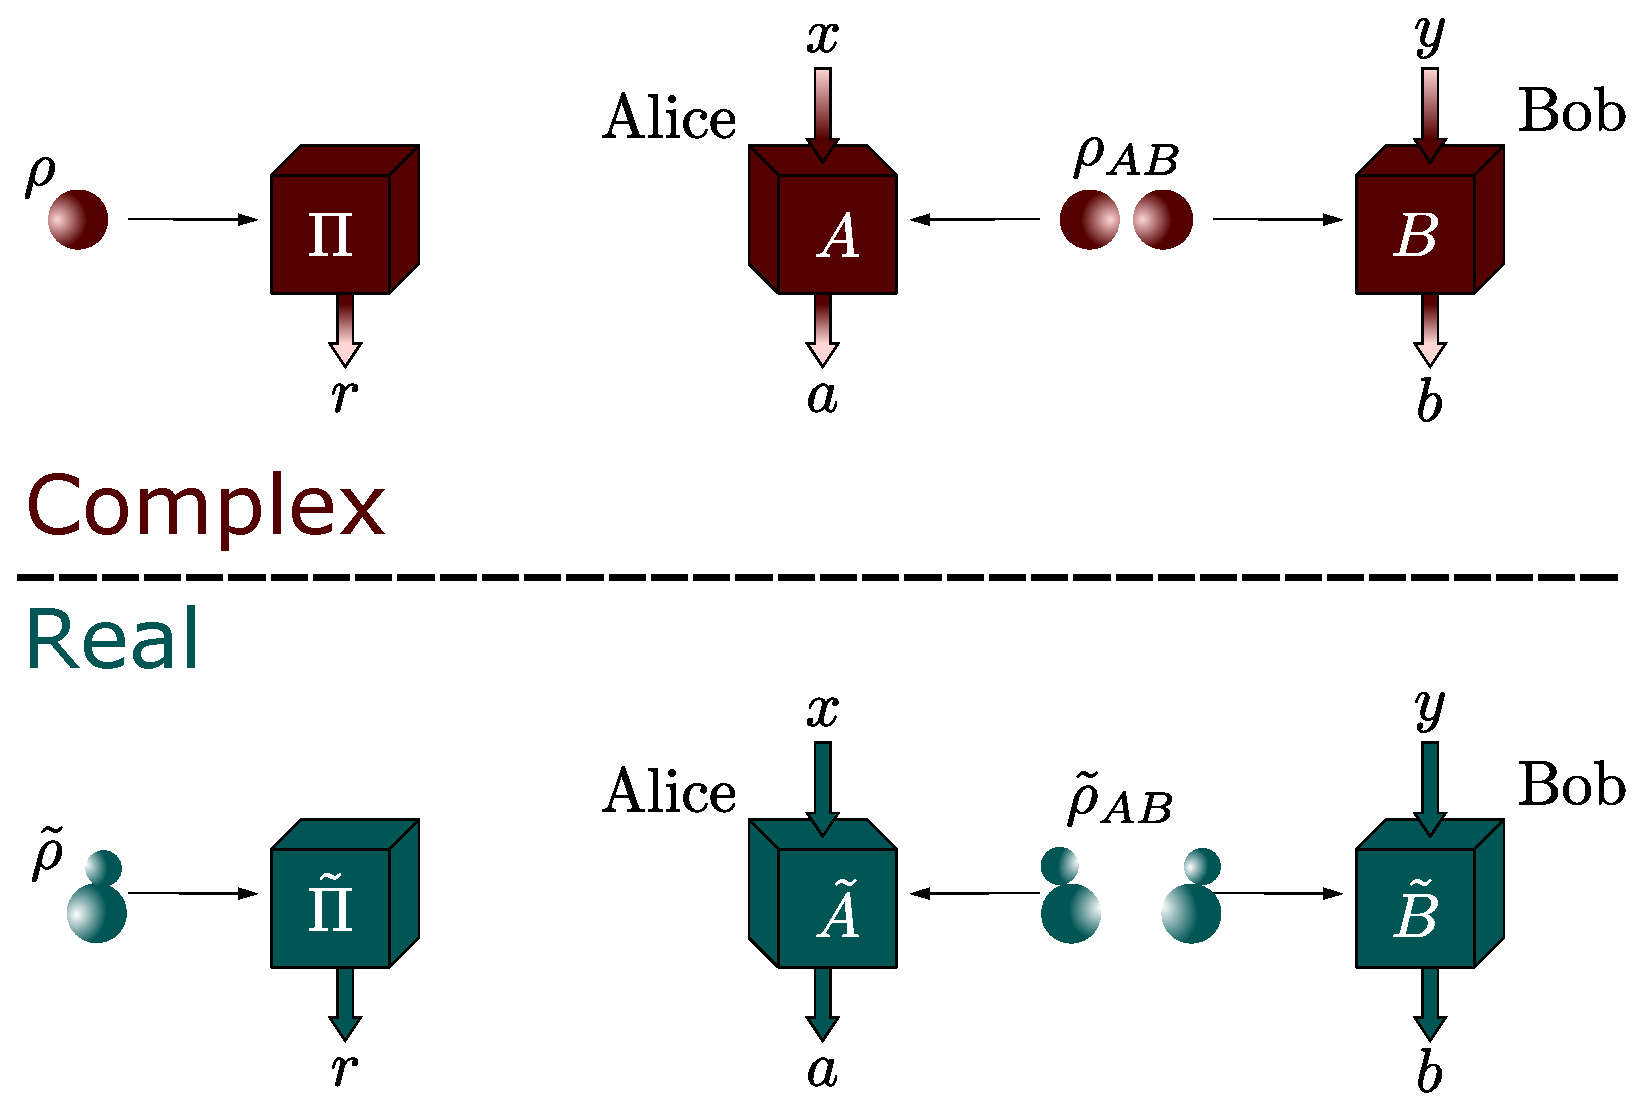
\includegraphics[width=12cm]{rvsc.pdf}
  \caption{\textbf{(Left pane) Single complex quantum system.} In standard quantum physics, a complex Hilbert space of dimension $d$ is associated to a system. The statistics of the experiment are computed from the system's state $\rho$ and measurement operators $\{\Pi_r\}_r$, wheres $r$ denotes the measurement outcome. To simulate the statistics using {\em real quantum physics}, an additional real qubit is added, effectively doubling the dimension. The state is replaced by the real state $\tilde{\rho}$ in Eq.~\eqref{eq:realstate}, while every measurement operator is replaced by the real measurement operator $\tilde\Pi_r=\Pi_r\otimes\proj{i}+\Pi_r^*\otimes\proj{-i}$. It is easy to see that $P(r)=\tr(\rho\Pi_r)=\tr(\tilde\rho\tilde\Pi_r)$. \textbf{(Right pane) Multipartite complex quantum system.} A standard Bell scenario consists of two particles distributed between Alice and Bob, who perform local measurements, labelled by $x$ and $y$, and get results $a$ and $b$. Complex Hilbert spaces of dimension $d_A$ and $d_B$ are assigned to each particle, while the joint Hilbert space of dimension $d_A\times d_B$ is defined by the tensor product of these. The state of the two particles is described by an operator $\rho_{AB}$ acting on the joint space, while operators $A_{a|x}$ and $B_{b|y}$ acting on each space describe the local measurements. The observed measurement statistics or correlations are described by the conditional probability distribution $P(ab|xy)=\tr(\rho_{AB}A_{a|x}\otimes B_{b|y})$. To simulate these statistics using {\em real quantum physics}, an extra real qubit is assigned to each particle, doubling each local dimension. The quantum state is replaced by the real state $\tilde \rho_{AA'BB'}$ in Eq.~\eqref{eq:realstateAB}, and the local measurements are replaced by the same transformation as before for a single system. The observed statistics is again recovered, i.e., $P(ab|xy)=\tr(\tilde\rho_{AB}\tilde{A}_{a|x}\otimes\tilde{B}_{b|y})$.}
  \label{fig:scenarios}
\end{figure}


Quantum predictions nonetheless become much more interesting when considering experiments involving several distant labs, where phenomena like entanglement \cite{schroedinger} and Bell non-locality \cite{Bell1964} can manifest. For the sake of simplicity, we focus on the case of two separate labs, although the results can easily be generalised to an arbitrary number of systems. In the considered Bell-type experiments, a source emits two particles (e.g.~a crystal pumped by a laser emitting two photons) in a state $\rho_{AB}$, each being measured by different observers, called Alice and Bob, see Fig.~\ref{fig:scenarios} (right pane). As pointed out by Bell \cite{Bell1964}, there exist quantum experiments where the observed correlations, encapsulated by the measured probabilities, %$\{P(a,b|x,y)\}$, or just $P(a,b|x,y)$ for short, 
are such that they cannot be reproduced by any local deterministic model, as they violate a Bell inequality. Such non-classical correlations are said to be \emph{nonlocal}, and their experimental realization disproves the universal validity of local classical physics. 
Is it possible that, like classical physics, real quantum physics can be falsified via a (complex) quantum Bell experiment? Note that if an experiment does not violate any Bell inequality, it is possible to reproduce the measured probabilities using a classical local deterministic model and, as said, real numbers suffice for classical physics. A Bell violation is therefore a necessary condition for a possible complex-real quantum gap. However, a Bell violation is not sufficient, as already exemplified by the famous Clauser-Horne-Shimony-Holt (CHSH) Bell inequality~\cite{chsh} $\text{CHSH}(1,2;1,2)=\langle A_1B_1\rangle +\langle A_1B_2\rangle+\langle A_2B_1\rangle-\langle A_2B_2\rangle\leq 2$. The inequality is derived for a Bell experiment where Alice and Bob perform two measurements with results $\pm 1$, and where $A_x$ ($B_y$) denote the results by Alice (Bob) when performing measurement $x=1,2$ ($y=1,2$). The maximal quantum violation of this inequality is $\beta_\text{CHSH}=2\sqrt 2$ and Alice and Bob can attain it using real measurements on a real two-qubit state.

To find a complex-real quantum gap, the ``complex" physicist might look for  Bell inequalities whose maximum quantum violations require complex numbers. Possible candidates are the elegant inequality of Ref.~\cite{elegant} or the combination of three CHSH inequalities introduced in~\cite{optimal_ent_bit,self_testing}
\begin{equation}
\label{eq:chsh3}
\text{CHSH}_3=\text{CHSH}(1,2;1,2)+\text{CHSH}(1,3;3,4)+\text{CHSH}(2,3;5,6)\leq 6,
\end{equation}
designed for a scenario in which Alice and Bob perform three and six measurements respectively, where the labels in the CHSH expressions denote the involved measurements. The maximal violation of the inequality is $3\beta_\text{CHSH}=6\sqrt 2$. With qubits, Alice and Bob obtain it in a natural way when they perform complex measurements on a two-qubit maximally entangled state. The three qubit measurements by Alice should be in three orthogonal spin directions, say $\sigma_z$, $\sigma_x$, and $\sigma_y$, which, in the $z$ basis, is an imaginary operator. 

However, none of these Bell inequalities will work: as shown in ~\cite{tamas_real, nicolas_real, moroder}, real quantum Bell experiments can reproduce the statistics of any quantum Bell experiment. Indeed, the construction of eq.~\eqref{eq:realstate} for single complex quantum systems can be adapted to the multipartite case if we allow the source to distribute an extra qubit for each observer, see Figure \ref{fig:scenarios} (right pane) for details. The resulting state is
\begin{equation}
\label{eq:realstateAB}
\tilde \rho_{AA'BB'} = \frac{1}{2}(\rho_{AB}\otimes\proj{+i,+i}_{A'B'} + \rho_{AB}^*\otimes\proj{-i,-i}_{A'B'}) .
\end{equation}
For years this was considered the final answer to our question: in quantum theory complex numbers are only convenient, but not necessary. Here we prove this conclusion wrong. 

For that purpose, we consider scenarios in which there is more than one source of entangled states distributed to several parties, who perform joint measurements. Such scenarios correspond to the future quantum internet, which will connect many quantum computers and guarantee quantum confidentiality over continental distances. In fact, while Bell experiments have earned considerable fame, they just represent a simple instance of a quantum network consisting of one source and many observers. It is now well understood that networks with richer geometries, in particular including more than one source, offer new perspectives for Bell-type demonstrations~\cite{bilocality,tobias1,tobias2,renouBSM,bancalBSM}. 
%%%%



To disprove real quantum physics, the ``complex" physicist proposes the network corresponding to a standard entanglement-swapping scenario, depicted in Fig.~\ref{fig:entswap}, consisting of two independent sources and three observers, Alice, Bob and Charlie. The two sources prepare two maximally entangled states of two qubits, the first one $\bar{\sigma}_{AB_1}$ distributed to Alice and Bob; and the second $\bar{\sigma}_{B_2C}$, to Bob and Charlie. Bob performs a standard Bell-state measurement on the two particles that he receives from the two sources. This measurement has the effect of swapping the entanglement from Alice and Bob and Bob and Charlie to Alice and Charlie: namely, for each of Bob's four possible outcomes, Alice and Charlie share a two-qubit entangled state. Note that the actual state depends on Bob's outcome, but not its degree of entanglement, which is always maximal. Alice and Charlie implement the measurements leading to the maximal violation of the $\text{CHSH}_3$ inequality~\eqref{eq:chsh3}. For these measurements, the state shared by Alice and Charlie, conditioned on Bob's result, maximally violates the inequality or a variant thereof produced by simple relabelings of the measurement outcomes.  

\begin{figure}
  \centering
  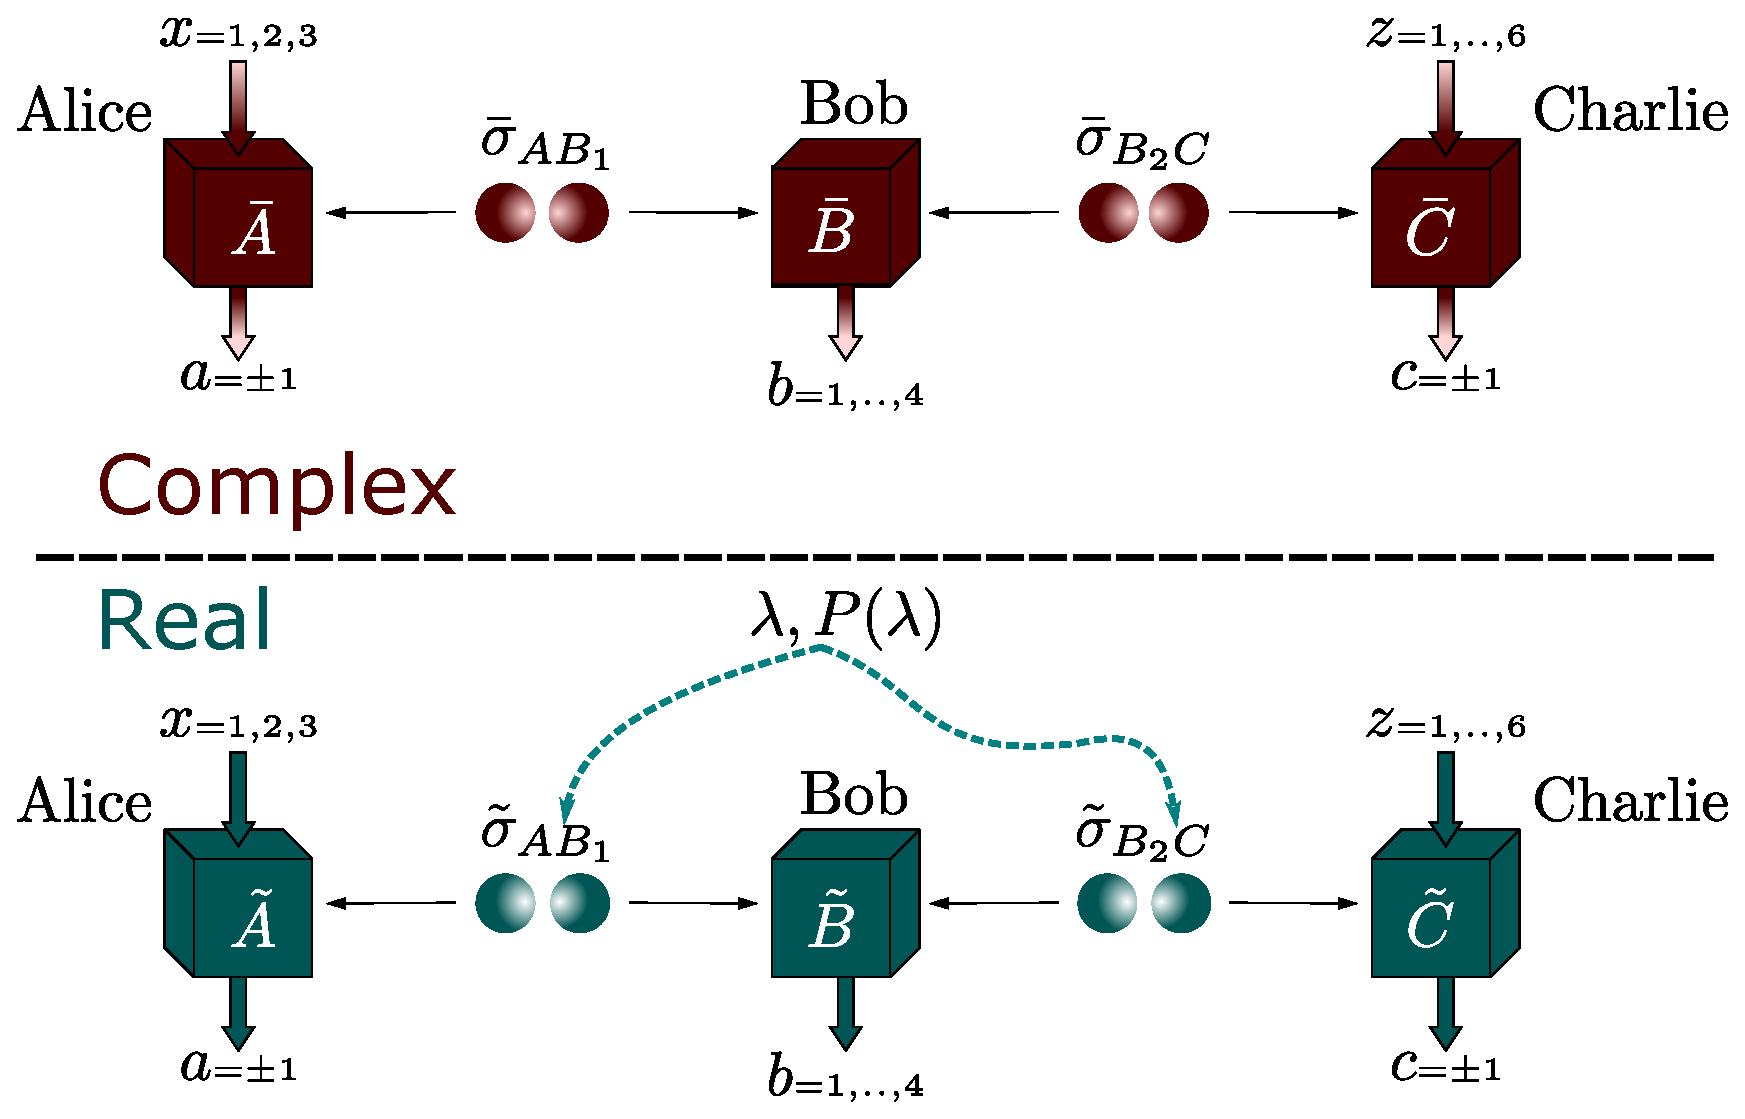
\includegraphics[width=15cm]{network.pdf}
  \caption{\textbf{Network scenario separating real and complex quantum physics.} In standard quantum physics (upper pane), two independent sources distribute the two-qubit states $\bar\sigma_{AB_1}$ and $\bar\sigma_{B_2C}$ to, respectively, Alice and Bob, and Bob and Charlie. At Bob's location, a Bell measurement, of four outputs, is implemented. Alice and Charlie apply the complex measurements leading to the maximal violation of the $\text{CHSH}_3$ inequality: three and six measurements with two possible outputs, labelled by $\pm 1$. According to quantum physics, the observed correlations read $P(abc|xz)=\tr\left((\bar{\sigma}_{AB_1}\otimes\bar{\sigma}_{B_2C})(\bar{A}_{a|x}\otimes\bar{B}_{b}\otimes\bar{C}_{c|z})\right)$. These correlations cannot be reproduced, or even well approximated, when all the states and measurements in the network are constrained to be real operators of arbitrary dimension (lower pane). The impossibility still holds if the two preparations are correlated through shared randomness (dashed mosque arrows), resulting in correlations of the form $P(abc|xz)=\sum_\lambda P(\lambda)\tr\left((\tilde\sigma_{AB_1}^\lambda\otimes\tilde\sigma_{B_2C}^\lambda)(\tilde{A}_{a|x}\otimes\tilde{B}_{b}\otimes\tilde{C}_{c|z})\right)$, where all operators are real.}
  \label{fig:entswap}
\end{figure}


It is intuitive that the previous real simulation strategy could not work in this scenario. Using just four outputs, the measurement by Bob should swap not only the entanglement in the states, but also the correlations in the extra flag qubits, so that Alice and Charlie perform the original measurements or their complex conjugates in a correlated way. Clearly, this only shows that a given strategy for real simulation does not work. However, it can be proven that no real simulation is indeed possible, that is, no real states and measurements can reproduce the statistics obtained in this entanglement swapping scenario. The proof, given in the Appendix, exploits the results of~\cite{self_testing}, where all quantum realisations leading to the maximal quantum value of~\eqref{eq:chsh3} were characterised. This characterization implies that any possible real simulation strategy attaining this maximal violation has to be with states of the form~\eqref{eq:realstateAB}. The proof follows by noting that, in this case, the marginal state shared by Alice and Charlie at the beginning of the experiment cannot be decomposed as a convex combination of real product states \cite{real_entanglement}. We moreover show the result to be robust, in the sense that the impossibility of real simulation also holds for non-maximal violations of the inequality~\eqref{eq:chsh3} between Alice and Charlie.

This result already solves our problem. However, in order to run an experiment and disprove the validity of real quantum physics, it is much more convenient to have an impossibility result phrased in terms of a Bell-type parameter, that is, a linear function of the observed correlations. To this end, we construct the Bell-type functional $\mathscr{T}$ defined by the sum of the violations of (the variants of) $\text{CHSH}_3$ inequality for each of Bob's measurement outputs, weighted by the probability of the output. In the ideal entanglement-swapping realisation with two-qubit maximally entangled states, the maximal quantum value of $\text{CHSH}_3$, equal to $6\sqrt 2$, is obtained for each of the four outputs by Bob, so $\mathscr{T}$ also attains its maximum quantum value, $\mathscr{T}=6\sqrt 2\approx 8.49$. Using a variant of the Navascu\'es-Pironio-Ac\'in (NPA) hierarchy~\cite{npa, npa2,NOP} introduced in~\cite{moroder}, we reduce the problem of upper bounding $\mathscr{T}$ over all real quantum realizations to a finite-dimensional convex optimization problem \cite{sdp}, that we solve numerically \cite{yalmip, mosek}, see the Appendix. In this way, we prove that, for real quantum systems, $\mathscr{T}\lesssim 7.66$. It is open, though, whether this upper bound is tight or the actual maximum value is even smaller. Since the map $\mathscr{T}$ is a linear function of the observed probabilities, the impossibility result holds even when the real simulation is assisted by shared randomness, see Fig.~\ref{fig:entswap} (lower pane). As shown in \cite{Elkouss}, \cite{Mateus}, this feature allows one to drop the assumption of independent and identical realizations in multiple-round hypothesis tests.

The setup needed to prove our results is very similar to the bilocality scenario described in~\cite{bilocality}, for which several experimental implementations have been reported~\cite{sciarrino,pryde,pan, Baumer2020}. Moreover, to beat the real bound on $\mathscr{T}$, one requires the two distributed states to have each a visibility beyond $\sqrt{7.66/6\sqrt 2}\sim 0.95$, a value attained in many experimental labs worldwide. The experiment similarly relies on the implementation of a challenging \cite{Bell_meas_impossible} but feasible \cite{Bell_meas_possible} two-qubit entangled measurement. All things considered, we believe that an experimental disproof of real quantum physics based on the inequality $\mathscr{T}$ is within reach using current technology. More details about the requirements for an experimental implementation are given in the Appendix.

Ever since the birth of modern science four centuries ago, abstract mathematical entities have played a big role in formalizing physical concepts. Our current understanding of velocity was only possible through the introduction of derivatives. The modern conception of gravity owes to the invention of non-Euclidean geometry. Basic notions from representation theory made it possible to formalize the notion of a fundamental particle. Here we considered whether the same holds for the complex numbers, originally introduced in mathematics to find the roots of cubic polynomials \cite{complex_numbers}. Somewhat surprisingly, we found that there do exist natural quantum scenarios that require the use of complex numbers to account for experimental observations. 

Our results rely on the assumption that the independence of two or more quantum systems is captured by the tensor product structure. If we drop this assumption, there exist real frameworks alternative to quantum theory that have the same predictive power, such as Bohmian mechanics \cite{Bohm} or real quantum physics with a universal qubit \cite{Aleksandrova_2013}. But when considering the standard quantum formalism, in which probabilities are computed through the Born rule and systems are composed through the tensor product, the use of complex or real numbers leads to different predictions. Our results are also robust and can be experimentally tested. We therefore trust that a disproof of real quantum physics will arrive in a near future.

From a broader point of view, our results advance the research program, started in~\cite{optimal_quantum}, of singling out quantum correlations by demanding maximal performance in a device-independent information-theoretic task. In this regard, our work shows that standard quantum physics outperforms real quantum physics when the non-local game $\mathscr{T}$ is played in the entanglement swapping scenario. This game can be interpreted as an extension of the adaptive CHSH game proposed in \cite{optimal_quantum}, which was recently shown to rule out a number of alternative physical theories in favor of quantum theory~\cite{optimal_quantum2b}. Whether the average score of $\mathscr{T}$ is maximized by standard quantum physics, or whether any physical theory other than standard quantum physics must necessarily produce a lower score are intriguing questions that we leave open.


\section*{Acknowledgements}
D.T. is a recipient of a DOC Fellowship of the Austrian Academy of Sciences at the Institute of Quantum Optics and Quantum Information (IQOQI), Vienna. L.P.T. is supported by the Lise Meitner Fellowship of the Austrian Academy of Sciences (project number M 2812-N). M.-O.R. and A.T. are supported by the Swiss National Fund Early Mobility Grants P2GEP2\_191444  and P2GEP2 194800 respectively. We acknowledge support from the Government of Spain (FIS2020-TRANQI and Severo Ochoa CEX2019-000910-S), Fundacio Cellex, Fundacio Mir-Puig, Generalitat de Catalunya (CERCA, AGAUR SGR 1381 and QuantumCAT), the ERC AdG CERQUTE, the AXA Chair in Quantum Information Science and the Swiss NCCR SwissMap.



\bibliography{rvsc_bib}

\newpage

\begin{appendix}

In this Appendix, we formally state and prove the results mentioned in the main text. It is organized as follows. In section \ref{sec:setup} we introduce the considered experimental scenario and state our main results, that we prove in sections \ref{sec:pbar}, \ref{sec:noisy} and \ref{numerics}. In section \ref{sec:experimental} we discuss the challenges and assumptions of a future experimental implementation.

\section{Setup and main results} \label{sec:setup}

Causal networks are the natural generalizations of Bell scenarios. In these experiments, several independent sources, quantum or classical, distribute physical systems that are probed by separate observers through quantum measurements. In this work, we consider the causal network depicted in Fig. \ref{fig:entswap} (lower pane). Alice and Bob are distributed the quantum state $\tilde{\sigma}_{AB_1}$, while Bob and Charlie are distributed the state $\tilde{\sigma}_{B_2C}$. These states might have been prepared using some shared randomness $\lambda$. Alice and Charlie can choose which measurement $x$ or $z$ to conduct, with results $a, c$. Bob, on the other hand, is just allowed to conduct a single measurement, with outcome $b$. This causal network is similar to an entanglement swapping setup and we therefore call it the \emph{SWAP scenario}. In the SWAP scenario, Alice, Bob and Charlie's observed behavior $P(a,b,c|x,z)$ must admit a decomposition of the form

\be
P(a,b,c|x,z)=\sum_\lambda P(\lambda)\tr\left\{(\tilde{\sigma}^{\lambda}_{AB_1}\otimes\tilde{\sigma}^{\lambda}_{B_2C})(\tilde{A}_{a|x}\otimes \tilde{B}_{b}\otimes \tilde{C}_{c|z})\right\},
\label{decomp}
\ee
\noindent for some quantum states $\tilde{\sigma}_{AB_1}^\lambda,\tilde{\sigma}_{B_2C}^\lambda$, some probability distribution $P(\lambda)$ and projective measurement operators $\tilde{A}_{a|x},\tilde{B}_{b},\tilde{C}_{c|z}$, with 

\be
\sum_{a}\tilde{A}_{a|x}=\id_A, \sum_b \tilde{B}_b=\id_B, \sum_c \tilde{C}_{c|z}=\id_C.
\ee

Notice that, in the SWAP scenario, it is no longer possible to use the real construction sketched in Figure \ref{fig:scenarios} (right pane). Indeed, in this scenario, any state shared between Alice and Charlie after tracing out Bob is a convex decomposition of product states, which are real if all quantum operations and states are assumed to be real. The construction in Figure \ref{fig:scenarios} (right pane), though, requires distributing Alice and Charlie the real quantum state $\frac{\rho\otimes\proj{i}^{\otimes 2}+\rho^*\otimes\proj{-i}^{\otimes 2}}{2}$. This state does not admit a \emph{real} separable decomposition, i.e., it cannot be expressed as a convex combination of tensor products of real quantum states. This can be seen by tracing the first part of the state and noticing that the resulting state, $\frac{\proj{i}^{\otimes 2}+\proj{-i}^{\otimes 2}}{2}$, despite being separable and real, cannot be written as a convex combination of real product states, as it is not invariant under the partial transposition of Alice's system~\cite{real_entanglement}.


The particular SWAP scenario we are interested in is one in which Alice and Charlie have, respectively, three, and six measurement settings, i.e., $x=1,2,3; z=1,...,6$. Both Alice's and Charlie's measurements are dichotomic, that is, $a,c=-1,1$. Bob's only measurement is assumed to have four outcomes $b=b_1b_2=00,01,10,11$, that we equivalently label as $b=\phi^+,\psi^+,\phi^-,\psi^-$ for reasons that will soon be obvious. 

In this scenario, let the two quantum sources respectively distribute to Alice and Bob and Bob and Charlie the states $\bar{\sigma}_{AB_1}=\bar{\sigma}_{B_2C}=\Phi^+=\proj{\phi^+}$, where $\ket{\phi^+}=\frac{1}{\sqrt{2}}(\ket{00}+\ket{11})$. We assume that Alice's three dichotomic observables $(\bar{A}_{1|x}-\bar{A}_{-1|x}:x=1,2,3)$ correspond to the three Pauli measurements $\sigma_Z,\sigma_X,\sigma_Y$, and that Charlie measures the dichotomic operators
\be
D_{ij}=\frac{\sigma_i+\sigma_j}{\sqrt{2}}, \qquad E_{ij}=\frac{\sigma_i-\sigma_j}{\sqrt{2}},
\ee
\noindent for $ij=zx,zy,xy$, which correspond to the observables $(\bar{C}_{1|x}-\bar{C}_{-1|x}:x=1,\ldots,6)$ when taken in the order $D_{zx}$, $E_{zx}$, $D_{zy}$, $E_{zy}$, $D_{xy}$, $E_{xy}$. Bob conducts a Bell basis measurement, with outcomes $b$ corresponding to each of the orthogonal projections onto the states $\ket{\phi^{\pm}}=\frac{1}{\sqrt{2}}(\ket{00}\pm\ket{11})$, $\ket{\psi^{\pm}}=\frac{1}{\sqrt{2}}(\ket{10}\pm\ket{01})$. We warn the reader that our convention of $\ket{\psi^-}$ differs from the usual one so as to make our formulas simpler. 

Call $\bar{P}=\{\bar{P}(a,b,c|x,z):a,b,c,x,z\}$ the resulting distribution. $\bar{P}$ obviously admits a representation of the form (\ref{decomp}), with \emph{complex} measurement operators. Since $\bar{P}$ does not require shared randomness $\lambda$ for its realization, it is also compatible with the less general causal network depicted in Figure \ref{fig:entswap} (upper pane).


Given some distribution $P(a,b,c|x,z)$, define $S^b_{xz}=\sum_{a,c=-1,1}P(a,b,c|x,z)ac$ and the linear functional

\begin{align}
\mathscr{T}_b(P)=& (-1)^{b_2}(S_{11}^b+S^b_{12})+(-1)^{b_1}(S^b_{21}-S^b_{22})+\nonumber\\
&(-1)^{b_2}(S^b_{13}+S^b_{14})-(-1)^{b_1+b_2}(S^b_{33}-S^b_{34})+\nonumber\\
& (-1)^{b_1}(S^b_{25}+S^b_{26})-(-1)^{b_1+b_2}(S^b_{35}-S^b_{36}).
\label{adjusted_3CHSH}
\end{align}
It can be verified that, for the considered states and measurements, the identity $\mathscr{T}_b(\bar{P})=6\sqrt{2}\bar{P}(b)$ holds for all $b$, with $\bar{P}(b)=\frac{1}{4}$. This means that, conditioned on any measurement outcome $b$ of Bob's, the state of Alice and Charlie's allows them to maximally violate one of the variants of the $\text{CHSH}_3$ Bell inequality, defined in eq. (\ref{eq:chsh3}).

Our first result, proven in section \ref{sec:pbar}, is the impossibility to reproduce $\bar{P}$ exactly using real quantum physics:

\begin{prop}
\label{exact_case}
$\bar{P}$ does not admit a decomposition of the form (\ref{decomp}) if we demand the states $\tilde{\sigma}_{AB_1}^\lambda,\tilde{\sigma}_{B_2C}^\lambda$ and measurement operators $\tilde{A}_{a|x},\tilde{B}_{b},\tilde{C}_{c|z}$ to be real.
\end{prop}

A more detailed argument, presented in section \ref{sec:noisy}, leads to the robustness claim:

\begin{theo}
\label{approximate_case}
Let $P(a,b,c|x,z)$ be a distribution such that $|P(b)-\frac{1}{4}|< \varepsilon_c$ and $\mathscr{T}_b(P)>(6\sqrt{2}-\varepsilon_c)P(b)$, for all $b$, with $\varepsilon_c\approx 1.3\cdot 10^{-4}$. Then, $P(a,b,c|x,z)$ does not admit a decomposition of the form (\ref{decomp}), with real states and measurement operators.
\end{theo}

Maximally violating the Bell inequality $\text{CHSH}_3$ with a precision of order $\varepsilon_c$ right after a Bell measurement is way beyond the capabilities of current quantum technologies. Define $\mathscr{T}(P)=\sum_{b\in\{0,1\}^2}\mathscr{T}_b(P)$, and note that in the considered setup $\mathscr{T}(\bar{P})=6\sqrt{2}\approx 8.4852$. 
In section \ref{numerics} we use ideas from non-commutative polynomial optimization \cite{NOP} to obtain the experimentally friendly robustness bound:


\begin{theo}
\label{main_theo}
For any distribution $P$ admitting a decomposition of the form (\ref{decomp}) with real quantum states and real measurement operators, 

\be
\mathscr{T}(P)\leq 7.6605.
\label{violation}
\ee
\end{theo}

\noindent The figure appearing in the theorem is the solution of a semidefinite program (SDP) \cite{sdp}, a type of convex optimization problem that can be solved in polynomial time. To arrive at this result, we used the SDP solver Mosek \cite{mosek}, with the MATLAB package YALMIP \cite{yalmip}. Note that, from duality theory, we can \emph{certify} that the solution of the SDP is the one stated in the theorem, up to computer precision. That is, the Theorem above represents a rigorous mathematical result, and can be understood as a computer-generated proof.


\section{Proof of Proposition \ref{exact_case}} \label{sec:pbar}
We prove the result by contradiction. Suppose that, indeed, there exist a distribution $P(\lambda)$, Hilbert spaces $A,B_1,B_2,C$, real states $\tilde{\sigma}_{AB_1}^\lambda,\tilde{\sigma}_{B_2C}^\lambda$ and real measurement operators $\tilde{A}_{a|x}, \tilde{B}_{b}, \tilde{C}_{c|z}$ such that eq.~\eqref{decomp} holds with $P=\bar{P}$. Let $\psi:=\sum_\lambda P(\lambda)\tilde{\sigma}^{\lambda}_{AB_1}\otimes\tilde{\sigma}^{\lambda}_{B_2C}$ be the global state for systems $A, B_1, B_2, C$ at the beginning of the experiment. With probability $P(b)=\tr(\psi \tilde{B}_b)$, Bob observes outcome $b$ and collapses the $AC$ system into the state $\tr_{B}(\tilde{B}_b \psi \tilde{B}_b)/P(b)$. We consider a real purification $\ket{\psi^b}$ of Alice and Charlie's conditional state, and redefine Charlie's system $C$ to accommodate the purifying system, over which Charlie's measurement operators act trivially. This is just to simplify our notation, i.e., to replace density matrices by kets. Since, at the end of the day, we will trace out the purifying system, whether such a purification physically exists or not does not affect the validity of the proof. We denote Alice's three dichotomic observables by $Z^A, X^A, Y^A$, referring to $(\tilde{A}_{1|x}-\tilde{A}_{-1|x}:x=1,2,3)$. Analogously, Charlie's dichotomic observables $(\tilde{C}_{1|z}-\tilde{C}_{-1|z}:z=1,...,6)$ are denoted by $D^C_{zx}, E^C_{zx}$, $D^C_{zy}$, $E^C_{zy}$, $D^C_{xy}$, $E^C_{xy}$, respectively.

\begin{figure}
\begin{center}
\centerline{
\Qcircuit @C=1em @R=1em{
 \lstick{A'} &\qw  & \gate{H} & \ctrl{2} \ar@{.}[]+<1.6em,1em>;[d]+<1.6em,-10.5em>    & \gate{H} & \ctrl{2} \ar@{.}[]+<1.6em,1em>;[d]+<1.6em,-10.5em> & \qw \ar@{.}[]+<2.3em,1em>;[d]+<2.3em,-10.5em>      & \qw  &  \qw\\
 \lstick{A''}& \qw & \gate{H} & \qw         & \qw      & \qw        & \ctrl{1}     & \gate{H} & \qw \\
 \lstick{A}  & \qw & \qw      & \gate{Z^A} & \qw       & \gate{X^A} & \gate{Y^AX^A} & \qw & \qw \\
 \lstick{C}  & \qw & \qw      & \gate{\hat{Z}^C} & \qw       & \gate{\hat{X}^C} & \gate{\hat{Y}^C\hat{X}^C} & \qw & \qw \\
 \lstick{C''}& \qw & \gate{H} & \qw         & \qw      & \qw        & \ctrl{-1}     & \gate{H} & \qw \\
 \lstick{C'} &\qw  & \gate{H} & \ctrl{-2}    & \gate{H} & \ctrl{-2}  & \qw            & \qw &  \qw\\
 & & & & & & & & \\
 & & {\text{Step 1}} & & { \qquad \ \text{Step 2}} & &  { \text{Step 3}} &   {\quad \ \text{Step 4}} & \\}}
\end{center}
\caption{Real local isometry $U\otimes V$ built from each party's untrusted measurement operators. For later reference, we denote the local isometry performing Steps 1 and 2 of the circuit as $U'\otimes V'$, and the remaining gates (performing the operations of Steps 3 and 4) as $U''\otimes V''$. The operators $\hat{X}^C$, $\hat{Y}^C$, $\hat{Z}^C$ are defined in terms of Charlie's measurement operators as the regularised versions of $X^C=\frac{D^C_{zx}-E^C_{zx}}{\sqrt{2}}$, $Y^C=\frac{D^C_{zy}-E^C_{zy}}{\sqrt{2}}$ and  $Z^C=\frac{D^C_{zx}+E^C_{zx}}{\sqrt{2}}$ respectively. $H$ denotes the Hadamard gate, defined through the relations $H\ket{0}=\frac{1}{\sqrt{2}}(\ket{0}+\ket{1})$, $H\ket{1}=\frac{1}{\sqrt{2}}(\ket{0}-\ket{1})$.
}
\label{isometry_pic}
\end{figure}

Taking inspiration from \cite{self_testing}, we consider the real isometry depicted in Figure \ref{isometry_pic}. Our first claim is that, if the real state $\ket{\psi^b}$ saturates the quantum bound $\bra{\psi^b}\mathscr{T}_b\ket{\psi^b}\leq 6\sqrt{2}$ for $b=\phi^+,\psi^+,\phi^-,\psi^-$, then the effect of this isometry on systems $A'A''C'C''$ is to prepare the states 
\begin{align} \label{eq:perfect_state}
\rho^b:= \tr_{AC}({U}\otimes {V} \ketbra{\psi^b}{\psi^b})=\ketbra{b}{b}\otimes\left[\frac{\Psi^++\Phi^-}{2}\right]_{A''C''}.
\end{align}
It can be verified that $\frac{\Psi^+ +\Phi^-}{2}=\frac{\proj{i}^{\otimes 2}+\proj{-i}^{\otimes 2}}{2}$. This shows that the real construction sketched in Figure \ref{fig:scenarios} (right pane) is somehow unavoidable: in order to simulate the statistics of Alice and Charlie (conditioned on Bob's outcome $b$), one needs to prepare the state $\frac{1}{2}(\proj{b}\otimes \proj{i}^{\otimes 2}+\proj{b}^*\otimes \proj{-i}^{\otimes 2})=\proj{b}\otimes \frac{\proj{i}^{\otimes 2}+\proj{-i}^{\otimes 2}}{2}$, as the construction requires.
We next prove eq. (\ref{eq:perfect_state}) for the case $b= \phi^+$; the other cases are completely analogous (or can be checked in Appendix~\ref{sec:noisy}). We explicitly show the effect of the isometry step by step. 
\begin{itemize}
\item After steps $1$ and $2$ of the isometry we are left with the state
\[
\ket{\psi^{\phi^+}}_{AC} \ket{0000}_{A'A''C'C''} \mapsto \ket{\phi^+}_{A'C'} \ket{+\!+}_{A''C''} \frac{\id + Z^A}{\sqrt{2}} \ket{\psi^{\phi^+}}_{{AC}}. 
\]
This follows from eq. (A12) in \cite{self_testing}, in turn a consequence of the maximal violation of the CHSH inequality through Alice and Charlie's first two measurement settings. We can now forget about systems $A'C'$, since the subsequent operations defining the isometry do not act on them. 

\item After Step $3$, systems ${A}A''{C}C''$ are in state
\begin{equation} \label{eq: middle state}
\frac{1}{2}(\ket{00}_{A''C''} \ket{\varphi}_{{AC}} + \ket{11}_{A''C''} Y^AX^A\hat{Y}^C \hat{X}^C \ket{\varphi}_{{AC}} + \ket{01}_{A''C''} \hat{Y}^C \hat{X}^C \ket{\varphi}_{{AC}}+\ket{10}_{A''C''} Y^AX^A \ket{\varphi}_{{AC}}),
\end{equation}
where $\ket{\varphi}_{{AC}}= \frac{\id+Z^A}{\sqrt{2}}\ket{\psi^{\phi^+}}_{{AC}}$. 
Since $\ket{\psi^{\phi^+}}$, maximally violates a $\text{CHSH}_3$ inequality, the identities 

\begin{align}
&\{X^A,Y^A\}_{+}\ket{\psi^{\phi^+}}_{{AC}}=\{X^A,Z^A\}_{+}\ket{\psi^{\phi^+}}_{{AC}}=\{Z^A,Y^A\}_{+}\ket{\psi^{\phi^+}}_{{AC}}=0,\nonumber\\
&\hat{Z}^C \ket{\psi^{\phi^+}}_{{AC}} = Z^A \ket{\psi^{\phi^+}}_{{AC}},\nonumber\\ 
&\hat{Y}^C \ket{\psi^{\phi^+}}_{{AC}} = -Y^A \ket{\psi^{\phi^+}}^{{AC}},\nonumber\\
&\hat{X}^C \ket{\psi^{\phi^+}}_{{AC}} = X^A \ket{\psi^{\phi^+}}_{{AC}}
\end{align}
\noindent hold, see \cite{self_testing} or Appendix C for a detailed proof. In turn, those imply the relations $\hat{Y}^C\hat{X}^C \ket{\varphi}_{{AC}} = Y^AX^A \ket{\varphi}_{{AC}}$ and $Y^A X^A\hat{Y}^C\hat{X}^C \ket{\varphi}_{{AC}} = - \ket{\varphi}_{{AC}}$.
Therefore \eqref{eq: middle state} is the same as 
\[
\frac{1}{\sqrt{2}} (\ket{\phi^-}_{A''C''} \ket{\varphi}_{{AC}} + \ket{\psi^+}_{A''C''} Y^A X^A \ket{\varphi}_{{AC}}).
\]

\item The Hadamard gates of step $4$ change $\ket{\phi^-}_{A''C''}$ to $\ket{\psi^+}_{A''C''}$ and viceversa. The final state is therefore
\[
\frac{1}{\sqrt{2}}\ket{\phi^+}_{A'C'}(\ket{\psi^+}_{A''C''} \ket{\varphi}_{{AC}} + \ket{\phi^-}_{A''C''} Y^A X^A \ket{\varphi}_{{AC}}).
\]
Finally, we take the partial trace over systems ${AC}$ to obtain
\[
\frac{1}{2} \Phi^+ \otimes \left(\bra{\varphi}Y^A X^A \ket{\varphi}(\ketbra{\phi^-}{\psi^+}+\ketbra{\psi^+}{\phi^-}) + \braket{\varphi}{\varphi} (\Psi^++\Phi^-)\right).
\]
Since $U\otimes V$ is an isometry, it immediately follows that $\braket{\varphi}{\varphi} = 1 $, which is equivalent to saying that $\bra{\psi^{\phi^+}}Z^A \ket{\psi^{\phi^+}}=0$. So far, all our considerations are general and did not use the fact that we are dealing with real numbers. Taking this fact into account, we have that
\[
\bra{\varphi} Y^A X^A \ket{\varphi} = \overline{\bra{\varphi} Y^A X^A \ket{\varphi}} = \bra{\varphi} X^A Y^A  \ket{\varphi} = - \bra{\varphi} Y^A X^A \ket{\varphi}.
\]
Therefore, this quantity is zero and the state left in systems $A'C'A''C''$ is indeed $\rho^b$.
\end{itemize}

Overall, summing over Bob's results, the application of ${ U}\otimes{ V}$ leaves system $A'A''C'C''$ in the state
\be
\rho=\sum_b \bar{P}(b)\rho^b=\frac{1}{4}\left(\rho^{\phi^+}+\rho^{\phi^-}+\rho^{\psi^+}+\rho^{\psi^-}\right)=\frac{\id_{A'C'}}{4}\otimes \left[\frac{\proj{i}^{\otimes 2}+\proj{-i}^{\otimes 2}}{2}\right]_{A''C''}.
\label{suma}
\ee


On the other hand, from (\ref{decomp}) we have that

\be
\rho=\sum_\lambda P(\lambda) \tr_A(U\tilde{\sigma}^\lambda_A U^\dagger)\otimes\tr_C(V\tilde{\sigma}^\lambda_C V^\dagger).
\ee
\noindent Since $\sigma_{A}^\lambda,\sigma_{C}^\lambda$ are real quantum states and $U, V$ are real quantum operations, it follows that $\rho$ must also be a real separable state. However, as we noted in Section~\ref{sec:setup}, the state $\frac{\proj{i}^{\otimes 2}+\proj{-i}^{\otimes 2}}{2}$ in systems $A''C''$ is \emph{not} real separable. Hence we reach a contradiction.


\section{Proof of Theorem \ref{approximate_case}} \label{sec:noisy}

First, we need to solve the optimization problem
\be
\min_{\tau \in \mathcal{S}}\norm{\tau-\rho_0}_1,
\label{optim_PT}
\ee
\noindent where $\mathcal{S}$ is the set of states in $A'A''B'B''$ invariant under transposition of $A'A''$ and $\rho_0=\rho$, as defined by the right-hand side of eq. (\ref{suma}).

Let $S_{A'A''}$ be the quantum channel defined by $S_{A'A''}(\bullet)=\sum_{\alpha',\alpha''=\pm i}\proj{\alpha'}\otimes\proj{\alpha''} \bullet \proj{\alpha'}\otimes\proj{\alpha''}$. Note that $S_{A'A''}^2=S_{A'A''}$, that $S_{A'A''}\otimes\id_{C'C''}(\rho_0)=\rho_0$ and that $S_{A'A''}\otimes\id_{C'C''}(\mathcal{S})\subset \mathcal{S}$. By the monotonicity of the trace norm, we thus have that $\tau$ in \eqref{optim_PT} can be chosen invariant under $S_{A'A''}\otimes\id_{C'C''}$. 

Any operator $O$ invariant under $S_{A'A''}\otimes\id_{C'C''}$ is of the form 

\be
O=\sum_{\alpha',\alpha''=\pm i}\proj{\alpha'}_{A'}\otimes\proj{\alpha''}_{A''}\otimes O^{\alpha',\alpha''}_{C'C''}.
\ee
\noindent It can be verified that the partial transposition of systems $A',A''$ of any such operator effects the transformation $O\to(\sigma^{\otimes 2}_z\otimes\id^{\otimes 2}) O(\sigma^{\otimes 2}_z\otimes\id^{\otimes 2})$. In particular, it does not change the operator's spectrum. It follows that, for any state $\tau\in \mathcal{S}$, invariant under $S_{A'A''}\otimes \id_{C'C''}$,

\be
\|\rho_0-\tau\|_1=\|\rho^{T_{AA'}}_0-\tau^{T_{AA'}}\|_1=\|\rho^{T_{A'A''}}_0-\tau\|_1.
\ee

\noindent Invoking the triangle inequality, we have that

\be
2=\|\rho_0-\rho^{T_{A'A''}}\|_1\leq \|\rho_0-\tau\|_1+\|\rho^{T_{A'A''}}_0-\tau\|_1=2\|\rho_0-\tau\|_1,
\ee
\noindent and hence the solution of problem (\ref{optim_PT}) is lower bounded by $1$. This bound happens to be tight: it is saturated by taking $\tau$ to be the maximally mixed state.

Having solved problem (\ref{optim_PT}), we proceed to prove Theorem \ref{approximate_case}. We use the same notation as in section \ref{sec:pbar}. Define $\omega:=(\tr_{B_1B_2}\psi)\otimes\ketbra{0000}{0000}_{A'C'A''C''}$ as Alice and Charlie's state before any measurement by Bob. Consider the state $\rho_\varepsilon:=\tr_{{AC}}(U\otimes V \omega U^T\otimes V^T)$ left on the $A'A''C'C''$ systems after applying over Alice and Charlie's systems ${AC}$ the real local isometries $U$, $V$ (see Figure~\ref{isometry_pic}) and tracing out ${AC}$.  As reasoned, such a state must be invariant under transposition of the systems $A'A''$ if Alice, Bob and Charlie's system admits a real quantum representation. Obviously, that will not happen if

\be
\norm{\rho_{\varepsilon}-\rho_0}_1 < \min_{\tau \in \mathcal{S}}\norm{\tau-\rho_0}_1=1.
\label{trace_norm_arg}
\ee

By the triangle inequality, we can bound
\begin{equation}\label{eq:normbnd}
\norm{\rho_{\varepsilon}-\rho_0}_1\leq \epsilon_1(\varepsilon)+\epsilon_2(\varepsilon),
\end{equation}
in terms of $\epsilon_1(\varepsilon) :=\norm{\rho_{\varepsilon}-\sum_b P(b) \sigma^b}_1$ and $\epsilon_2(\varepsilon) :=\norm{\sum_b P(b) \sigma^b-\rho_0}_1$, where $\sigma^b= \tr_{{AC}}(\ketbra{\sigma^b}{\sigma^b})$ and $\ket{\sigma^b}$ are the potentially {\em unnormalized} states

\begin{align}\label{sigma}
    \ket{\sigma^b} = 
    \begin{cases}
    \ket{\phi^+}\otimes\frac{1}{\sqrt{2}}\left[\ket{\psi^+}\frac{\id+Z^A}{\sqrt{2}}\ket{\psi^b} + \ket{\phi^-}Y^AX^A\frac{\id+Z^A}{\sqrt{2}}\ket{\psi^b}\right] & \text{ for } b = 00 = \phi^+\\
    \ket{\psi^+}\otimes\frac{1}{\sqrt{2}}\left[\ket{\psi^+}\frac{X^A(\id-Z^A)}{\sqrt{2}}\ket{\psi^b} + \ket{\phi^-}\frac{Y^A(\id-Z^A)}{\sqrt{2}}\ket{\psi^b}\right] & \text{ for } b = 01 = \psi^+\\
    \ket{\phi^-}\otimes\frac{1}{\sqrt{2}}\left[\ket{\psi^+}\frac{\id+Z^A}{\sqrt{2}}\ket{\psi^b} + \ket{\phi^-}Y^AX^A\frac{\id+Z^A}{\sqrt{2}}\ket{\psi^b}\right] & \text{ for } b = 10 = \phi^-\\
    \ket{\psi^-}\otimes\frac{1}{\sqrt{2}}\left[\ket{\psi^+}\frac{X^A(\id-Z^A)}{\sqrt{2}}\ket{\psi^b} + \ket{\phi^-}\frac{Y^A(\id-Z^A)}{\sqrt{2}}\ket{\psi^b}\right] & \text{ for } b = 11 = \psi^-.
    \end{cases}
\end{align}
Thus, if the sum of the upper bounds on $\epsilon_1(\varepsilon)$ and $\epsilon_2(\varepsilon)$ computed in the following sections is smaller than $1$, then, by eq. (\ref{trace_norm_arg}), $\rho_\varepsilon$ is not reproducible with real quantum states. This leads to a critical error value of $\varepsilon_c = 1.3 \cdot 10^{-4}$.



\subsection{Upper bounds on $\epsilon_1(\varepsilon)$}

%Let $b=(b_1,b_2)$ with $b_1, b_2 \in \{0,1\}$ define the four inequalities 
%\begin{equation}
%\begin{aligned}
%    \mathscr{T}(b)=(-1)^{b_2}Z^A(D_{z,x}^C+E_{z,x}^C)&+(-1)^{b_1}X^A(D_{z,x}^C-E_{z,x}^C)+\\
%    (-1)^{b_2}Z^A(D_{z,y}^C+E_{z,y}^C)& - (-1)^{b_1+b_2}Y^A(D_{z,y}^C-E_{z,y}^C)+\\
%    (-1)^{b_1}X^A(D_{x,y}^C+E_{x,y}^C)& - (-1)^{b_1+b_2}Y^A(D_{x,y}^C-E_{x,y}^C)\leq6\sqrt{2}.
%\end{aligned}
%\end{equation}


\begin{lem} \label{lem1} Let  $\ket{\psi}$ be a state that, with the measurement operators $X^A$, $Y^A$, $Z^A$ for Alice and $D^C_{xy}$, $D^C_{zx}$, $D^C_{zy}$, $E^C_{xy}$, $E^C_{zx}$, $E^C_{zy}$ for Charlie, obeys $\bra{\psi}\mathscr{T}_b\ket{\psi}=6\sqrt{2}-\varepsilon$, then
\begin{align}
    \norm{U\otimes V\left(\ket{\psi}_{{AC}}\ket{0000}_{A'C'A''C''}\right) - \ket{\sigma^b}}  \leq  (10.5+11\sqrt{2}+(\sqrt{2})^{-1})\varepsilon_1,
    \label{eps2}
\end{align}
with $\varepsilon_1=\sqrt{\sqrt{2}\varepsilon}$ and where $U \otimes V$ denotes the isometry from Figure~\ref{isometry_pic} with $\hat{X}^C$, $\hat{Y}^C$, $\hat{Z}^C$ the regularised versions of $\frac{D^C_{zx}-E^C_{zx}}{\sqrt{2}}$, $\frac{D^C_{zy}-E^C_{zy}}{\sqrt{2}}$ and  $\frac{D^C_{zx}+E^C_{zx}}{\sqrt{2}}$ respectively.
\end{lem}


\begin{proof}
%Given $\bra{\psi}\mathscr{T}(b)\ket{\psi}=6\sqrt{2}-\varepsilon$ with $\ket{\psi}\equiv\ket{\psi^b}$ the post-selected {\em normalized} state after Bob observed the outcome $b$, 
Let us first define the regularised operators
\begin{align}
    \hat Z^C := \text{reg}(Z^C) \equiv \text{reg}(Z^C_{zx}), \text{ similarly for } X^C \equiv X^C_{zx} \text{ and } Y^C\equiv Y^C_{zy},
\end{align}
where the regularization procedure, as used in~\cite{self_testing}, turns a bounded operator into a unitary operator and 
\begin{align}
    Z^C_{zx}:=\frac{D^C_{zx}+E^C_{zx}}{\sqrt{2}}, X^C_{zx}:=\frac{D^C_{zx}-E^C_{zx}}{\sqrt{2}}\\
    Z^C_{zy}:=\frac{D^C_{zy}+E^C_{zy}}{\sqrt{2}}, Y^C_{zy}:=\frac{D^C_{zy}-E^C_{zy}}{\sqrt{2}}\\
    X^C_{xy}:=\frac{D^C_{xy}+E^C_{xy}}{\sqrt{2}}, Y^C_{xy}:=\frac{D^C_{xy}-E^C_{xy}}{\sqrt{2}}
\end{align}
Note that these definitions are independent of $b$. Then using the sum-of-square (SOS) decomposition
\begin{align}
    \sqrt{2}(6\sqrt{2}-\mathscr{T}_b)&=\left[(-1)^{b_2}Z^A-\frac{D^C_{zx}+E^C_{zx}}{\sqrt{2}}\right]^2 + \left[(-1)^{b_1}X^A-\frac{D^C_{zx}-E^C_{zx}}{\sqrt{2}}\right]^2\\
    &+\left[(-1)^{b_2}Z^A-\frac{D^C_{zy}+E^C_{zy}}{\sqrt{2}}\right]^2 + \left[(-1)^{b_1+b_2}Y^A+\frac{D^C_{zy}-E^C_{zy}}{\sqrt{2}}\right]^2\\
    &+\left[(-1)^{b_1}X^A-\frac{D^C_{xy}+E^C_{xy}}{\sqrt{2}}\right]^2 + \left[(-1)^{b_1+b_2}Y^A+\frac{D^C_{xy}-E^C_{xy}}{\sqrt{2}}\right]^2.
\end{align}
we read off the following approximate relations
\begin{equation}\label{eq:CtoA}
\norm{((-1)^{b_2}Z^A-Z^C)\ket{\psi}}, \ \norm{((-1)^{b_1}X^A-X^C)\ket{\psi}}, \ \norm{((-1)^{b_1+b_2}Y^A+Y^C)\ket{\psi}} \leq \varepsilon_1\,.
\end{equation}

By using the SOS decomposition
\begin{align}
\sqrt{2}(6\sqrt{2}\id -\mathscr{T}(b)) &= \left[D^C_{zx}- \frac{(-1)^{b_2}Z^A+(-1)^{b_1}X^A}{\sqrt{2}}\right]^2+\left[E^C_{zx} - \frac{(-1)^{b_2}Z^A-(-1)^{b_1}X^A}{\sqrt{2}} \right]^2 \nonumber \\
&+ \left[D^C_{zy} - \frac{(-1)^{b_2}Z^A-(-1)^{b_1+b_2}Y^A}{\sqrt{2}}\right]^2+\left[E^C_{zy} - \frac{(-1)^{b_2}Z^A+(-1)^{b_1+b_2}Y^A}{\sqrt{2}} \right]^2 \nonumber \\
&+ \left[D^C_{xy} - \frac{(-1)^{b_1}X^A-(-1)^{b_1+b_2}Y^A}{\sqrt{2}}\right]^2+\left[E^C_{xy} - \frac{(-1)^{b_1}X^A+(-1)^{b_1+b_2}Y^A}{\sqrt{2}} \right]^2 \label{sos2}
\end{align}
we can read off
\begin{equation}\label{eq:anticomm_approx}
    \norm{\{(-1)^{b_2}Z^A,(-1)^{b_1}X^A\}\ket{\psi}}, \ \norm{\{(-1)^{b_2}Z^A,(-1)^{b_1+b_2}Y^A\}\ket{\psi}}, \ \norm{\{(-1)^{b_1+b_2}Y^A,(-1)^{b_1}X^A\}\ket{\psi}} \leq (1+\sqrt{2})\varepsilon_1,
\end{equation}
i.e., $X^A,Y^A,Z^A$ all anticommute approximately.


Finally, the regularized operators are also close to the unregularized counterparts, e.g.
\begin{equation}\label{eq:reg_approx}
    \norm{(\hat Z^C-Z^C)\ket{\psi}}=\norm{(\id-(\hat Z^C)^\dagger Z^C)\ket{\psi}}=\norm{(\id-\abs{Z^C})\ket{\psi}}=\norm{(\id-\abs{Z^AZ^C})\ket{\psi}}\leq\norm{(\id-Z^AZ^C)\ket{\psi}}\leq\varepsilon_1.
\end{equation}

Now we apply the isometry $U\otimes V$ defined in Figure~\ref{isometry_pic}. The cancellation happens exactly as in the ideal case  incurring a small loss measured in vector norm because relations are only approximate. After $U'\otimes V'$ (see Figure~\ref{isometry_pic}), the unknown state is close to a (potentially unnormalized) vector in a specific form
\begin{equation}
    \norm{U'\otimes V'(\ket{\psi}_{{AC}}\ket{00}_{A'C'})-\mathcal{O}(b)\ket{\psi}_{{AC}}\ket{b}_{A'C'}} \leq (4.5+(\sqrt{2})^{-1})\varepsilon_1
\end{equation}
where
\begin{equation}
    \mathcal{O}(b)=\begin{cases}
    \frac{\id+Z^A}{\sqrt{2}} & \text { if } b_2=0\\
    \frac{X^A(\id-Z^A)}{\sqrt{2}} & \text { if } b_2=1
    \end{cases}
\end{equation}
To get this result, we compute the effect of the different steps of the isometry on the initial vector and make use of the relations \eqref{eq:CtoA}, \eqref{eq:anticomm_approx}, \eqref{eq:reg_approx} in order to simplify the final expression, all the while keeping track of the error incurred to at each stage. That is, we first apply the Hadamard gates, and then control $Z^A$ and $\hat Z^C$ gates, which return a state as written in the first line of Step 1 below. Since so far we did not use any of the approximate relations, the error incurred to in this step is $0$, as written on the left of the state in Step 1. Next, we use the approximate relation \eqref{eq:CtoA} to convert $Z^A\hat Z^C\ket{\psi}$ to $(-1)^{b_2}Z^AZ^A\ket{\psi}=(-1)^{b_2}\ket{\psi}$, and similarly $\hat Z^C\ket{\psi}$ to $\hat Z^A\ket{\psi}$, incurring into an error $2\varepsilon_1$, written on the left. Continuing this way through the circuit, the intermediate expressions, together with their bounds, are the following:
\begin{align*}
  \text{Step 1:} \qquad \qquad 0\varepsilon_1: & \frac{1}{2}\left[\ket{00}+\ket{11}Z^A\hat Z^C+\ket{01}\hat Z^C+\ket{10}Z^A\right]\ket{\psi}\\
    2\varepsilon_1: & \frac{1}{2}\left[(\ket{00}+(-1)^{b_2}\ket{11})\id+((-1)^{b_2}\ket{01}+\ket{10})Z^A\right]\ket{\psi}\\
  \text{Step 2:} \qquad \qquad 0\varepsilon_1: & \frac{1}{4}\Big[\ket{00}(1+(-1)^{b_2})(\id+Z^A)+\ket{11}(1+(-1)^{b_2})X^A\hat X^C(\id-Z^A)+\\
    \, & \quad \quad \ket{01}(1-(-1)^{b_2})\hat X^C(\id+Z^A)+\ket{10}(1-(-1)^{b_2})X^A(\id-Z^A)]\Big]\ket{\psi}\\
    (5+\sqrt{2})\varepsilon_1/2: & \frac{1}{4}\left[(1+(-1)^{b_2})(\ket{00}+(-1)^{b_1}\ket{11})(\id+Z^A) + (1-(-1)^{b_2})((-1)^{b_1}\ket{01}+\ket{10})X^A(\id-Z^A)]\right]\ket{\psi}
\end{align*}
Note that in the last approximation, the two paths $b_2=0$ and $b_2=1$ have the same upper bound. Also, we use the convention that $\ket{\psi^-}=(\ket{10}-\ket{01})/\sqrt{2}$, which has the same density matrix as the usual convention.

The rest of the circuit does not involve $A'C'$ so we can safely ignore them. After the remaining local unitaries $U''\otimes V''$ (see Figure~\ref{isometry_pic}), 
\begin{equation}
\norm{U''\otimes V''\left(\mathcal{O}(b)\ket{\psi}_{{AC}}\ket{00}_{A''C''}\right) - \ket{\tau^b}} \leq (6+11\sqrt{2})\varepsilon_1,
\end{equation}
where
\begin{align}
    \ket{\tau^b}=
    \begin{cases}
    \frac{1}{\sqrt{2}}\left[\ket{\psi^+}\frac{\id+Z^A}{\sqrt{2}}\ket{\psi} + \ket{\phi^-}Y^AX^A\frac{\id+Z^A}{\sqrt{2}}\ket{\psi}\right] & \text{ for } b_2 = 0\\
    \frac{1}{\sqrt{2}}\left[\ket{\psi^+}\frac{X^A(\id-Z^A)}{\sqrt{2}}\ket{\psi} + \ket{\phi^-}\frac{Y^A(\id-Z^A)}{\sqrt{2}}\ket{\psi}\right] & \text{ for } b_2 = 1
    \end{cases}
\end{align}
The intermediate steps are
\begin{align*}
  \text{Step 3:} \qquad \qquad  \qquad 0\varepsilon_1 : & \frac{1}{2}\left[\ket{00}\mathcal{O}(b) + \ket{11}Y^AX^A\hat Y^C\hat X^C\mathcal{O}(b) + \ket{01}\hat Y^C\hat X^C\mathcal{O}(b) + \ket{10}Y^AX^A\mathcal{O}(b)\right]\ket{\psi}\\
    (4+8\sqrt{2})\varepsilon_1: & \frac{1}{2}\left[\ket{00}\mathcal{O}(b)  + \ket{11}Y^AX^AY^AX^A\mathcal{O}(b) +  \ket{01}Y^A X^A\mathcal{O}(b) + \ket{10}Y^AX^A\mathcal{O}(b)\right]\ket{\psi}\\
    (2+3\sqrt{2})\varepsilon_1: & \frac{1}{2}\left[(\ket{00} - \ket{11})\mathcal{O}(b) + (\ket{01} + \ket{10})Y^AX^A\mathcal{O}(b)\right]\ket{\psi}\\
   \text{Step 4:} \qquad \qquad  \qquad 0\varepsilon_1: & \frac{1}{2}\left[(\ket{01}+\ket{10})\mathcal{O}(b) + (\ket{00}-\ket{11})Y^AX^A\mathcal{O}(b)\right]\ket{\psi}
\end{align*}
where we have taken the larger bound among the two $b_2=1$ and $b_2=0$ cases to get
\begin{align}
    \norm{(\hat Y^C\hat X^C\mathcal{O}(b) - Y^AX^A\mathcal{O}(b))\ket{\psi}} &\leq (16+4\sqrt{2})\varepsilon_1/\sqrt{2} \text{ and }\\
    \norm{(Y^AX^AY^AX^A\mathcal{O}(b) + \mathcal{O}(b))\ket{\psi}} &\leq (6+2\sqrt{2})\varepsilon_1/\sqrt{2}\,.
\end{align}

By a series of triangle inequalities going through all the intermediate expressions, we get the Lemma.
%\begin{align}
%    \norm{U\otimes V\left(\ket{\psi}^{AC}\ket{0000}^{A'C'A''C''}\right) - \ket{\sigma^b}}  \leq  (10.5+11\sqrt{2}+(\sqrt{2})^{-1})\varepsilon_1.
%    \label{eps2}
%\end{align}
%where for $\ket{\psi}\equiv\ket{\psi^b}$ the subnormalized state per our convention,
%\begin{align}\label{eq: state}
%    \ket{\sigma^b} = \ket{b}^{A'C'}\otimes\ket{\tau^b}^{ACA''C''} = 
%    \begin{cases}
%    \ket{\Phi^+}\otimes\frac{1}{\sqrt{2}}\left[\ket{\Psi^+}\frac{\id+Z^A}{\sqrt{2}}\ket{\psi} + \ket{\Phi^-}Y^AX^A\frac{\id+Z^A}{\sqrt{2}}\ket{\psi}\right] & \text{ for } b = 00 = \Phi^+\\
%    \ket{\Psi^+}\otimes\frac{1}{\sqrt{2}}\left[\ket{\Psi^+}\frac{X^A(\id-Z^A)}{\sqrt{2}}\ket{\psi} + \ket{\Phi^-}\frac{Y^A(\id-Z^A)}{\sqrt{2}}\ket{\psi}\right] & \text{ for } b = 01 = \Psi^+\\
%    \ket{\Phi^-}\otimes\frac{1}{\sqrt{2}}\left[\ket{\Psi^+}\frac{\id+Z^A}{\sqrt{2}}\ket{\psi} + \ket{\Phi^-}Y^AX^A\frac{\id+Z^A}{\sqrt{2}}\ket{\psi}\right] & \text{ for } b = 10 = \Phi^-\\
%    \ket{\Psi^-}\otimes\frac{1}{\sqrt{2}}\left[\ket{\Psi^+}\frac{X^A(\id-Z^A)}{\sqrt{2}}\ket{\psi} + \ket{\Phi^-}\frac{Y^A(\id-Z^A)}{\sqrt{2}}\ket{\psi}\right] & \text{ for } b = 11 = \Psi^-
 %   \end{cases}
%\end{align}
\end{proof}

\begin{lem} \label{lem2} Let $\ket{\sigma^b}$ be any state defined in \eqref{sigma} and let $\varepsilon_1=\sqrt{\sqrt{2}\varepsilon}$, then
\begin{equation}\label{eq:lem2}
1-\frac{5+\sqrt{2}}{2}\varepsilon_1 \leq \norm{\ket{\sigma^b}}^2 \leq 1 + \frac{5+\sqrt{2}}{2}\varepsilon_1.
\end{equation}
\end{lem}

\begin{proof}
With $\norm{\ket{\sigma^b}}^2 = \tr{\proj{\sigma^b}}$ then
\be\label{eq:lem2b}
\abs{1-\tr{\proj{\sigma^b}}} = \abs{\bra{\psi^b} Z^A \ket{\psi^b}}.
\ee

\noindent  Now consider, as in \cite{singlet},
\begin{align*}
\abs{\bra{\psi^b}Z^A \ket{\psi^b}+\bra{\psi^b}Z^A X^A \hat{X}^C \ket{\psi^b}}
&=\abs{\bra{\psi^b}Z^A \ket{\psi^b}+\bra{\psi^b}\hat{X}^C X^A Z^A \ket{\psi^b}}\\
 &= \abs{\bra{\psi^b}(\hat{X}^C Z^A \hat{X}^C + \hat{X}^C X^A Z^A) \ket{\psi^b}} \\
&\leq \norm{\hat{X}^C \ket{\psi^b}} \norm{(Z^A \hat{X}^C +X^A Z^A) \ket{\psi^b}} \leq  (3+\sqrt{2})\varepsilon_1. \\
\abs{\bra{\psi^b}Z^A \ket{\psi^b}-\bra{\psi^b}Z^AX^A\hat{X}^C \ket{\psi^b}} &\leq \norm{(Z^A(\id - X^A \hat{X}^C)\ket{\psi^b}}\\
& \leq \norm{Z^A(\hat{X}^C-X^A) \ket{\psi^b}} \leq 2\varepsilon_1,
\end{align*}
where we used the Cauchy-Schwarz inequality as well as 
\[
\norm{(Z^A\hat{X}^C+ X^AZ^A) \ket{\psi^b}} \leq \norm{(Z^A\hat{X}^C-Z^AX^A)\ket{\psi^b}} + \norm{\{X^A,Z^A\}\ket{\psi^b}} \leq 2\varepsilon_1+(1+\sqrt{2})\varepsilon_1.
\]
Therefore, we find that \begin{equation}\label{ZA}
 \abs{\bra{\psi^b} Z^A \ket{\psi^b}}\leq \frac{5+\sqrt{2}}{2}\varepsilon_1,   
\end{equation} which combined with \eqref{eq:lem2b} implies \eqref{eq:lem2}.
\end{proof}

\bigskip

\noindent Using these Lemmas, we can obtain the final bound for $\epsilon_1(\varepsilon)$. Firstly, we have
\begin{equation}
\epsilon_1(\varepsilon) \leq \sum_b P(b) \norm{\ketbra{\rho_\varepsilon^b}{\rho_\varepsilon^b}-\ketbra{\sigma^b}{\sigma^b}}_1  \leq  2 \sum_b P(b) \sqrt{
\frac{(1+\norm{\ket{\sigma^b}}^2)^2}{4}-\abs{\braket{\rho_\varepsilon^b}{\sigma^b}}^2},
\end{equation}
where the first equality comes from $\rho_\varepsilon=\sum_b P(b) \rho_\varepsilon^b$ for $\rho_\varepsilon^b$ the $A'C'A''C''$ marginal of the state $\ket{\rho_\varepsilon^b}=U\otimes V(\ket{\psi^b}_{AC}\ket{0000}^{A'C'A''C''})$.
The last inequality follows by adapting an argument from~\cite{Watrous} to non-normalised states. Namely, since $\ketbra{\rho_\varepsilon^b}{\rho_\varepsilon^b}-\ketbra{\sigma^b}{\sigma^b}$ has rank at most two,
\begin{alignat}{2}
\lambda_1+\lambda_2&= \  \tr(\ketbra{\rho_\varepsilon^b}{\rho_\varepsilon^b}-\ketbra{\sigma^b}{\sigma^b}) &&= 1- \norm{\ket{\sigma^b}}^2 \nonumber\\
\lambda_1^2+\lambda_2^2 &= \ \tr((\ketbra{\rho_\varepsilon^b}{\rho_\varepsilon^b}-\ketbra{\sigma^b}{\sigma^b})^2) &&= 1+ \norm{\ket{\sigma^b}}^4-2\abs{\braket{\rho_\varepsilon^b}{\sigma^b}}^2, \nonumber
\end{alignat}
where $\lambda_1$ and $\lambda_2$ are the two eigenvalues of $\ketbra{\rho_\varepsilon^b}{\rho_\varepsilon^b}-\ketbra{\sigma^b}{\sigma^b}$. We can thus compute
$$\abs{\lambda_1}+\abs{\lambda_2}=\sqrt{2(\lambda_1^2+\lambda_2^2)-(\lambda_1+\lambda_2)^2}= 2\sqrt{
\frac{(1+\norm{\ket{\sigma^b}}^2)^2}{4}-\abs{\braket{\rho_\varepsilon^b}{\sigma^b}}^2}. $$


\noindent Furthermore, 
\[
\braket{\rho_\varepsilon^b}{\sigma^b} = \frac{1+\norm{\ket{\sigma^b}}^2-\norm{\ket{\rho_\varepsilon^b}-\ket{\sigma^b}}^2}{2} 
\]
which implies, by Lemma~\ref{lem1} and Lemma~\ref{lem2}, that for small $\varepsilon > 0$,
\[
\epsilon_1(\varepsilon) \leq 2\sqrt{\frac{(1+(1+\frac{5+ \sqrt{2}}{2} \varepsilon_1))^2}{4}-\left(1- \frac{(5+\sqrt{2})\varepsilon_1/2 + \varepsilon_2^2}{2} \right)^2},
\]
where we set $\varepsilon_2:=(10.5+11\sqrt{2}+(\sqrt{2})^{-1})\varepsilon_1$.




\subsection{Upper bounds on $\epsilon_2(\varepsilon)$ }

To bound $\epsilon_2(\varepsilon)=\|\sum_b P(b)\sigma^b-\rho_0\|_1$, let us first separate the expression in the norm as 
\begin{align*}
\norm{\sigma^{b}-\rho_0^{b}}_1 &\leq \abs{\hat{\mu}(b)} \norm{\proj{b}\otimes(\ketbra{\phi^-}{\psi^+}+\ketbra{\psi^+}{\phi^-})}_1 + \abs{\mu(b)} \norm{\proj{b}\otimes(\proj{\phi^-}+\proj{\psi^+})}_1, \\
%&= \frac{1}{2}(3+\sqrt{2})\varepsilon_1+\frac{1}{2}(4\varepsilon_1 + (1+\sqrt{2})\varepsilon_1) = (4+\sqrt{2})\varepsilon_1
\end{align*}
where the coefficients simplify to $
\abs{\mu(b)} = \frac{1}{2} \abs{\bra{\psi^b} Z^A \ket{\psi^b}}$
and 
\begin{align*}
 \abs{\hat{\mu}(b)} =\begin{cases}
  \frac{1}{4} \abs{\bra{\psi^b} (\id + Z^A) X^A Y^A(\id + Z^A) \ket{\psi^b}} & b_2=0 \\ 
  \frac{1}{4} \abs{\bra{\psi^b} (\id - Z^A) X^A Y^A(\id - Z^A) \ket{\psi^b}} & b_2=1. \\
 \end{cases}  
\end{align*} 

\noindent To bound $\abs{\hat{\mu}(b)}$, let us consider
\begin{align}
 \frac{1}{4} \abs{\bra{\psi^b} (\id + (-1)^{b_2} Z^A)\{X^A, Y^A\}(\id + (-1)^{b_2} Z^A) \ket{\psi^b}} & \leq \frac{1}{4}\norm{(\id+ (-1)^{b_2} Z^A)\ket{\psi^b}}\norm{\{X^A, Y^A\}(\id + (-1)^{b_2}  Z^A) \ket{\psi^b}}  \nonumber \\
&\leq \frac{1}{2} \norm{\{X^A, Y^A\}(\id + (-1)^{b_2} Z^A) \ket{\psi^b}} \nonumber \\
& \leq \frac{1}{2} (\norm{\{X^A, Y^A\}\ket{\psi^b}} \nonumber\\
&+ \norm{\hat{Z}^C\{X^A, Y^A\} \ket{\psi^b}} + \norm{\{X^A, Y^A\}(Z^A-\hat{Z}^C)\ket{\psi^b}}) \nonumber \\
& \leq  ((1+\sqrt{2})\varepsilon_1 + 2 \varepsilon_1).\label{eq:b1}
\end{align}

\noindent Therefore, using \eqref{eq:b1} and \eqref{ZA}, we obtain
\begin{align*}
\norm{\sigma^{b}-\rho_0^{b}}_1 &\leq 
 \frac{1}{2}(3+\sqrt{2})\varepsilon_1+\frac{1}{2}(4\varepsilon_1 + (1+\sqrt{2})\varepsilon_1) = (4+\sqrt{2})\varepsilon_1 .
\end{align*}

\noindent Since $\abs{P(b)-\frac{1}{4}} \leq \varepsilon$, we obtain 
\begin{align}
\epsilon_2(\varepsilon) \leq \sum_b \frac{1}{4} \norm{\sigma^b-\rho_0^b}_1 + \sum_b \abs{P(b)-\frac{1}{4}} \norm{ \sigma^b }_1\leq (4+\sqrt{2})\varepsilon_1 + 4 \left( 1 + \frac{5+\sqrt{2}}{2}\varepsilon_1\right) \varepsilon.
\end{align}

\section{Proof of Theorem \ref{main_theo}}
\label{numerics}

 
Our first step is to obtain a tractable necessary condition for a distribution $P$ to admit a real quantum realization. To this aim, we invoke the essentials of non-commutative polynomial optimization \cite{NOP}.

Let $P$ admit a real quantum representation of the form (\ref{decomp}), and think of an abstract unital $\star$-algebra ${\cal A}$ with generators $A_{1|1},A_{1|2},A_{1|3}$, together with the relations $A_{1|x}=A_{1|x}^\dagger=(A_{1|x})^2$, for $x=1,2,3$. We consider the natural isomorphism $\pi_A$ that maps any element of ${\cal A}$ to the algebra generated by the operators $\{\tilde{A}_{1|x}:x=1,2,3\}$. That is, $A_{1|x}$ is an element of ${\cal A}$, while $\pi_A(A_{1|x})=\tilde{A}_{1|x}$ represents Alice's physical measurement operator for setting $x$ and outcome $a=1$. We call $\A\subset {\cal A}$ the set of all monomials of degree $n_A$ or lower of $A_{1|1},A_{1|2},A_{1|3}\in {\cal A}$ including the identity, for some fixed natural number $n_A$. Similarly, we define an abstract unital $\star$-algebra ${\cal C}$ with projection generators $C_{1|1},...,C_{1|6}$ to model Charlie's measurements, with the natural isomorphism $\pi_C$. We denote by $\C\subset{\cal C}$ the set of all monomials of degree $n_C$ or lower of $C_{1|1},...,C_{1|6}$, including the identity for some fixed $n_C$.


Following Moroder \emph{et al.}'s interpretation \cite{moroder} of the Navascu\'es-Pironio-Ac\'in (NPA) hierarchy \cite{npa, npa2}, to each monomial $\alpha\in {\cal A}$ we associate a normalized ket $\ket{\alpha}$ such that $\braket{\alpha'}{\alpha}=\delta_{\alpha,\alpha'}$, for all $\alpha,\alpha'\in{\cal A}$. Likewise, we associate an orthonormal basis to the set ${\cal C}$. Next, we define the completely positive local maps $\Omega_A$, $\Omega_C$ through the relations:

\begin{align}
&\Omega_A(\eta)=\sum_{\alpha,\alpha'\in\A} \tr\left((\pi_A(\alpha)^{\dagger}\eta \pi_A(\alpha')\right)\ket{\alpha}\bra{\alpha'}\nonumber\\
&\Omega_C(\eta)=\sum_{\gamma,\gamma'\in \C} \tr\left(\pi_C(\gamma)^\dagger\eta \pi_C(\gamma')\right)\ket{\gamma}\bra{\gamma'}.
\end{align}

\noindent $\Omega_A$ ($\Omega_C$) thus maps states in Alice's (Charlie's) untrusted system $A$ ($C$) to a non-normalized state with support in $H_A=\mbox{span}\{\ket{\alpha}:\alpha\in\A\}$ ($H_C=\mbox{span}\{\ket{\gamma}:\gamma\in \C\}$).

For $\lambda\in\Lambda$, define the state $\tilde{\omega}^b(\lambda)\equiv\tr_{B_1B_2}\left\{(\tilde{\sigma}_{AB_1}^\lambda\otimes \tilde{\sigma}_{B_2C}^\lambda)(\id_A\otimes \tilde{B}_b\otimes\id_C)\right\}$ and consider the $|\A||\C|\times |\A||\C|$ matrix

\be
\Gamma^b\equiv \sum_\lambda P(\lambda)(\Omega_A\otimes\Omega_C)(\tilde{\omega}^b(\lambda)).
\ee
\noindent Since $\Omega_A,\Omega_C$ are completely positive, this matrix must be positive semidefinite. Moreover, some of its entries are related. Indeed, let the monomials $\alpha_1,...,\alpha_4\in\A$, $\gamma_1,...,\gamma_4\in\C$ be such that $\alpha_2\alpha_1^\dagger=\alpha_4\alpha_3^\dagger=:\alpha$, $\gamma_2\gamma_1^\dagger=\gamma_4\gamma_3^\dagger=:\gamma$. Then it holds that

\be
\bra{\alpha_1}\bra{\gamma_1}\Gamma^b\ket{\alpha_2}\ket{\gamma_2}=\bra{\alpha_3}\bra{\gamma_3}\Gamma^b\ket{\alpha_4}\ket{\gamma_4}=\sum_{\lambda} P(\lambda)\tr\{\tilde{\omega}^b(\lambda) (\pi_A(\alpha)\otimes\pi_C(\gamma))\}.
\label{basic_identity}
\ee
\noindent This allows us to write $\Gamma^b$ as

\be
\Gamma^b=\sum_{\alpha\in\A\cdot\A,\gamma\in\C\cdot\C}d^b_{\alpha,\gamma}M^{\alpha}\otimes N^{\gamma},
\label{gammas}
\ee
\noindent where $\{d^b_{\alpha,\gamma}:\alpha,\gamma\}$ are real coefficients, and, for any $a,a'\in\A, c,c'\in\C$, the corresponding entries of $M^{\alpha}$, $N^{\gamma}$ are given by

\be
M^\alpha_{a,a'}=\delta_{\alpha, a'a^\dagger},N^\gamma_{c,c'}=\delta_{\gamma,c'c^\dagger}.
\ee
\noindent Also, notice that some of the coefficients $d^b_{\alpha,\gamma}$ follow from the experimental data $P(a,b,c|x,z)$. Namely, 

\be
d^b_{\id,\id}=P(b),d^b_{A_{1|x},\id}=P_{AB}(1,b|x),d^b_{\id,C_{1|z}}=P_{BC}(b,1|z),d^b_{A_{1|x},C_{1|z}}=P(1,b,1|x,z).
\label{probas}
\ee
\noindent In the terminology of \cite{NOP}, $\Gamma^b$ is a non-normalized \emph{moment matrix} for the distribution $P(a,c|x,z, b)$, with norm $d^b_{\id,\id}=P(b)$.

Consider now the matrix $\Gamma\equiv\sum_b\Gamma^b$. From the definition of $\tilde{\omega}^b(\lambda)$, we have that, for any $\lambda\in\Lambda$, $\sum_b\tilde{\omega}^b(\lambda)=\tilde{\sigma}^\lambda_A\otimes \tilde{\sigma}^\lambda_C$. It follows that

\be
\Gamma=\sum_{\lambda}P(\lambda)\Omega_A(\tilde{\sigma}^\lambda_A)\otimes\Omega_C(\tilde{\sigma}^\lambda_C).
\ee
Since $\Omega_A, \Omega_C$ are real completely positive maps, we have that $\Gamma$ is a real separable operator, i.e., a conic combination of real product quantum states. In particular, it must be that $\Gamma$ equals its partial transpose, $\Gamma^{T_A}=\Gamma$ \cite{real_entanglement}.

To summarize: if $P$ admits a real quantum representation in the SWAP scenario, then there must exist real coefficients $d^b_{\alpha,\gamma}$ such that eq. (\ref{probas}) holds, the matrices $\Gamma^b$ defined through eq. (\ref{gammas}) are positive semidefinite and the matrix $\sum_{b}\Gamma^b$ is its own partial transpose. Consider then the following optimization problem:

\begin{align}
\max_{d, P} \quad &\mathscr{T}(P),\nonumber\\
\mbox{such that } \quad &\Gamma^b=\sum_{\alpha\in\A\cdot \A,\gamma\in\C\cdot \C}d^b_{\alpha,\gamma}M^\alpha\otimes N^\gamma\geq 0,\mbox{ for }b=1,...,4,\nonumber\\
&(\sum_b\Gamma^b)^{T_A}=\sum_b\Gamma^b,\nonumber\\
&d^b_{\id,\id}=P(b),d^b_{A_{1|x},\id}=P_{AB}(1,b|x),d^b_{\id,C_{1|z}}=P_{BC}(b,1|z),d^b_{A_{1|x},C_{1|z}}=P(1,b,1|x,z),\nonumber\\
&P(a,b,c|x,z)\geq 0, \sum_{a}P(a,b,c|x,z)=P_{BC}(b,c|z),\sum_{c}P(a,b,c|x,z)=P_{AB}(a,b|x),\nonumber\\&\sum_aP_{AB}(a,b|x)=\sum_cP_{BC}(b,c|z)=P(b), \sum_b P(b)=1,
\end{align}
\noindent where the conditions on $P(a,b,c|x,z)$ in the last two lines enforce that $P$ corresponds to a non-signalling, normalized tripartite distribution.

The above is a semidefinite program (SDP) \cite{sdp}, and, as long as the matrices $M^\alpha,N^\gamma$ are not very large, one can find the solution in a normal desktop. Since the constraints enforce a relaxation of the requirement that $P$ admit a representation in the SWAP scenario, it follows that the solution of this problem is an upper bound on the maximum value of $\mathscr{T}(P)$ for $P$ achievable through real quantum systems in the considered causal structure.

Taking $n_A=n_C=2$, and using the SDP solver MOSEK \cite{mosek} within the optimization package YALMIP \cite{yalmip}, we arrive at Theorem \ref{main_theo}.



\section{Experimental considerations}
\label{sec:experimental}

In view of Theorem \ref{main_theo}, there exists a considerable gap between the predictions of real and complex quantum theory in the entanglement swapping scenario. Does that mean that an actual experimental refutation of real quantum theory is within reach? Let us briefly consider how an experimental realization of the quantum experiment depicted in Figure \ref{fig:entswap} (up) would go. 

First, a general observation: even if our experimental setup mimics that of Figure \ref{fig:entswap}, in principle, there could exist prior quantum correlations between the two preparation devices, or a quantum state shared by the three parties as a result of a past quantum interaction (say, in the last round of experiments). In either predicament, our previous bounds on the input-output statistics for real quantum system would not be valid, and any claims of refutation of real quantum physics would be unfounded. These two possibilities, though, rely on the presence of hidden quantum memories within the experimental equipment. Hence, if we posit a time-scale beyond which the devices' quantum memories degrade into classical information, we can discard such contingencies just by spacing out the experimental rounds sufficiently (note that prior classical correlations between the parties can be absorbed into the definition of $\lambda$). 

There is another loophole, namely, the possible existence of hidden state sources that distribute general tripartite entangled states at each experimental round. This quagmire, that would similarly compromise the conclusions of the experiment, cannot be ruled out by appealing to decoherence or space-like separation. In order to refute real quantum physics, we are thus compelled to accept some plausible, yet unverifiable, assumptions about the form of the quantum states distributed to the three parties. In the following, we therefore \emph{postulate} that Figure \ref{fig:entswap} (down) accurately captures the causal scenario encountered by the three parties at each experimental round. Crucially, we allow the states $\tilde{\sigma}_{AB_1}^{\lambda}, \tilde{\sigma}_{B_2C}^\lambda$ and the distribution $P(\lambda)$ to depend in arbitrary ways on the past history $h$ of measurement settings and outcomes observed by the three parties in the course of the experiment. That is, we allow the real quantum physicist to adapt its states and measurement operators at each round to make us believe that it holds complex quantum resources.

Under the above adversarial conditions, the inequality $\mathscr{T}\leq 7.6605$ nonetheless holds at every experimental round. Therefore, one can use the techniques in \cite{Elkouss} and \cite{Mateus} to devise an $n$-round experiment that, if successful, disproves the hypothesis of real quantum physics with high statistical confidence.

Of course, in order to get there, one first needs to realize a quantum entanglement swapping experiment with $\mathscr{T}>7.6605$. We next discuss the technical feasibility of this goal. We assume that $\bar{\sigma}_{AB},\bar{\sigma}_{BC}$ are distributed via photon sources, and that photon polarization measurements are almost perfect. We then face two experimental problems: making sure that the photons reach their destination more or less unperturbed and conducting the Bell measurement. With regards to the first problem, we model the interaction between the photons and the environment through white noise. That is, rather than being distributed two maximally entangled states, Alice and Bob and Bob and Charlie respectively receive an independent copy of the state $v\Phi^++\frac{1-v}{4}\openone$. Under ideal Bell measurements, the violation of the inequality $\mathscr{T}\leq 7.6605$ thus requires each photon source to have a visibility $v$ of at least $v=\sqrt{\frac{7.6005}{6\sqrt{2}}}\approx 0.95$. With regards to the second problem, deterministic Bell-state measurements with photons are indeed complicated \cite{Bell_meas_impossible}, but they can be carried out with arbitrary precision, provided that sufficiently many single-photon sources are available \cite{Bell_meas_possible}. All in all, the experimental requirements to violate (\ref{violation}) are demanding, but not unreasonably so.


\end{appendix}


\end{document}
